%%%%%%%%%%%%%%%%%%%%%%%%%%%%%%%%%%%%%%%%%%%%%%%%%%%%%%%%%%%%%%%%%%%%%%%%%%%%%%%%%%%%%%%%%%%%%%%%%%%
%%%%%%%%%%%%%%%%%%%%%%%%%%%%%%%%%%%%%%%%%%%%%%%%%%%%%%%%%%%%%%%%%%%%%%%%%%%%%%%%%%%%%%%%%%%%%%%%%%%
%%%%%%%%%%%%%%%%%%%%%%%%%%%%%%%%%%%%%%%%%%%%%%%%%%%%%%%%%%%%%%%%%%%%%%%%%%%%%%%%%%%%%%%%%%%%%%%%%%%
%%%%%%%%%%%%%%%%%%%%%%%%%%%%%%%%%%%%%%%%%%%%%%%%%%%%%%%%%%%%%%%%%%%%%%%%%%%%%%%%%%%%%%%%%%%%%%%%%%%

\chapter{Resultados}

En cada canal que conforma el PSG (EEG, EOG y EMG), cada \'epoca registrada fue clasificada como 
'posiblemente estacionaria' (PE) si, usando la prueba PSR, no pudo rechazarse la hip\'otesis de 
estacionariedad ($\alpha < 0.05$), o como 'no-estacionaria' en caso contrario.
La cantidad de \'epocas PE en cada individuo, durante el sue\~no MOR y NMOR, se muestra en las 
tablas \ref{total_gpos_mor}, \ref{total_gpos_nmor} y \ref{total_gpos_total}. Debido a la gran 
variabilidad entre los sujetos para la duraci\'on del sue\~no MOR, no se consider\'o el total de 
\'epocas PE, sino la proporci\'on de \'estas en cada etapa de sue\~no; tales cantidades se muestran 
en las tablas \ref{gpos_mor}, \ref{gpos_nmor} y \ref{gpos_total}. 
Adicionalmente se han calculado promedios y desviaciones est\'andar para ambos grupos (Control y 
PDC).

\section{Resultados principales}

Como un primer an\'alisis se verific\'o si el sue\~no MOR, entendido como muestra del registro
completo, tiene o no propiedades estad\'isticas parecidas a este \'ultimo, y si \'esta similaridad 
pudiera estar relacionada con el PDC. 
Se compar\'o la proporci\'on de \'epocas PE en cada canal durante sue\~no MOR y NMOR usando la 
prueba $\chi^{2}$ para proporciones\footnote{Implementada en R como la funci\'on 
\texttt{prop.test()}}; estos resultados se muestran en la tabla \ref{comparacion_mor_vs_total},
y son resumidos esquem\'aticamente en la figura \ref{cabecitas_munchas}.

Se encontr\'o que no hay diferencias significativas, consistentes en todos los sujetos, en los 
canales LOG y ROG, lo cual puede ser explicado por la tipificaci\'on del sue\~no MOR. 
Por otro lado, no se encontr\'o una relaci\'on clara entre el estado de salud del sujeto y la 
aparici\'on de diferencias significativas entre estas proporciones.

\begin{figure}
\centering
\begin{tabular}{c}
\begin{tabular}{ccccc}
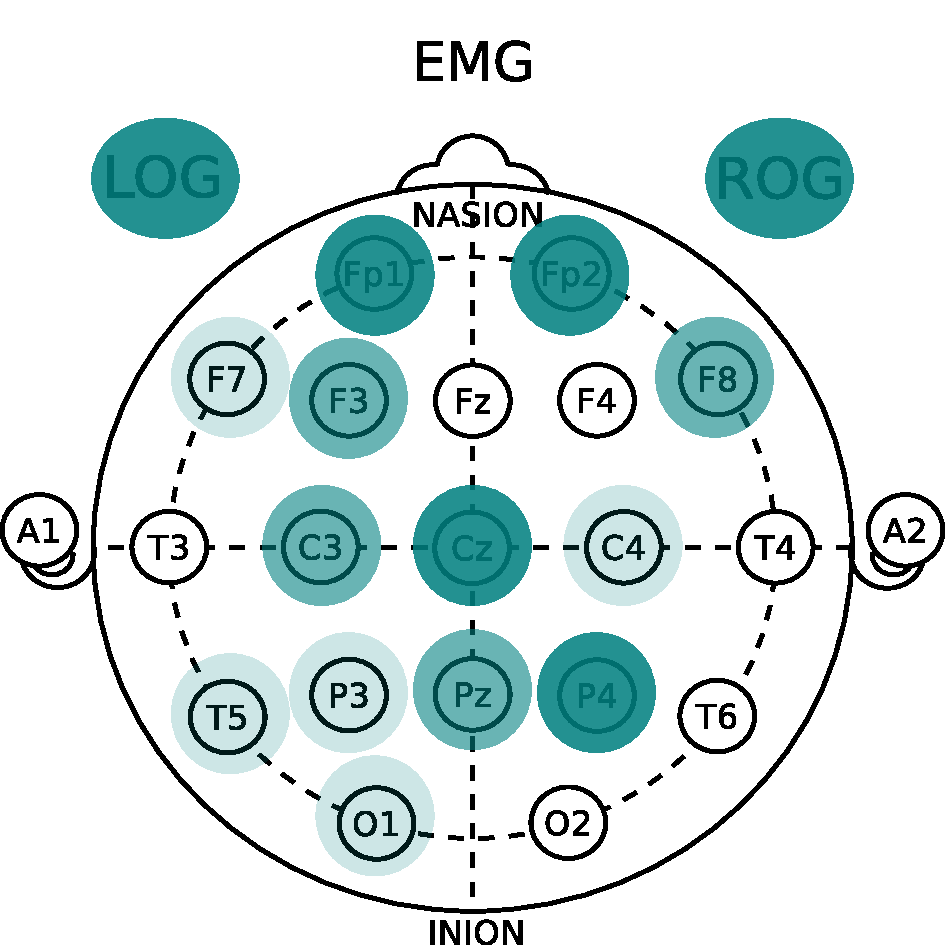
\includegraphics[width=0.17\textwidth]{./img_diagramas/cabecita_VCR.pdf} &
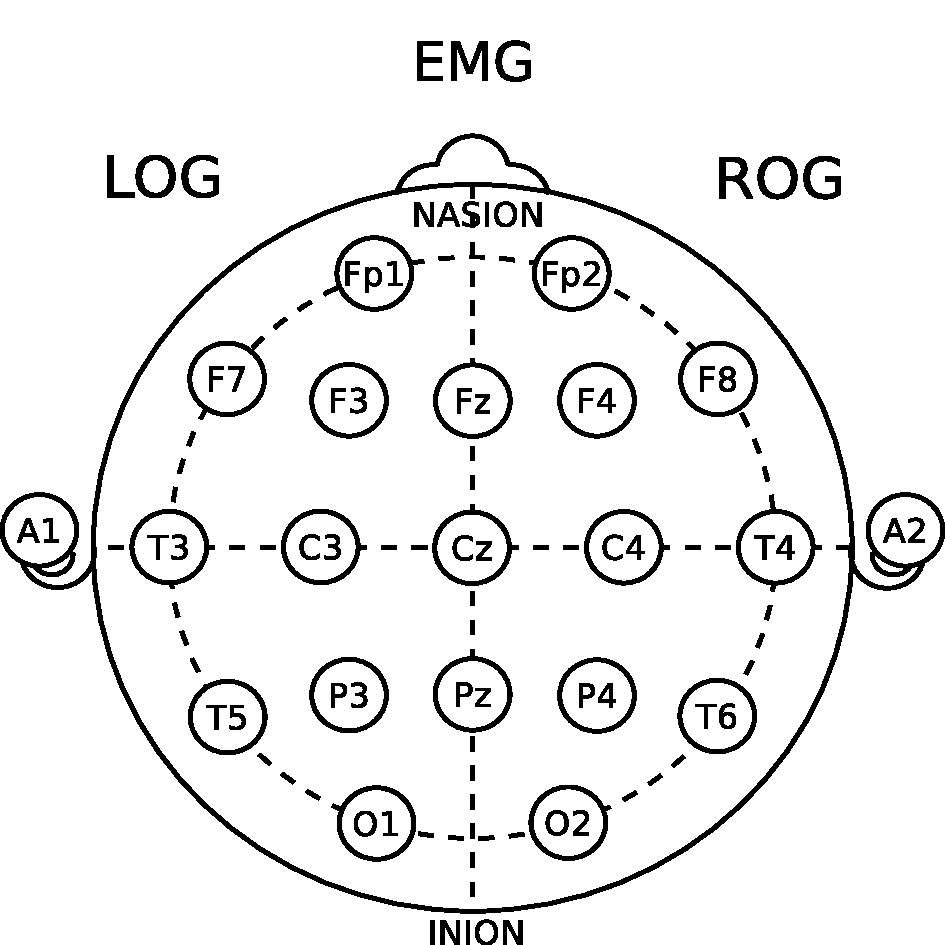
\includegraphics[width=0.17\textwidth]{./img_diagramas/cabecita_MJH.pdf} &
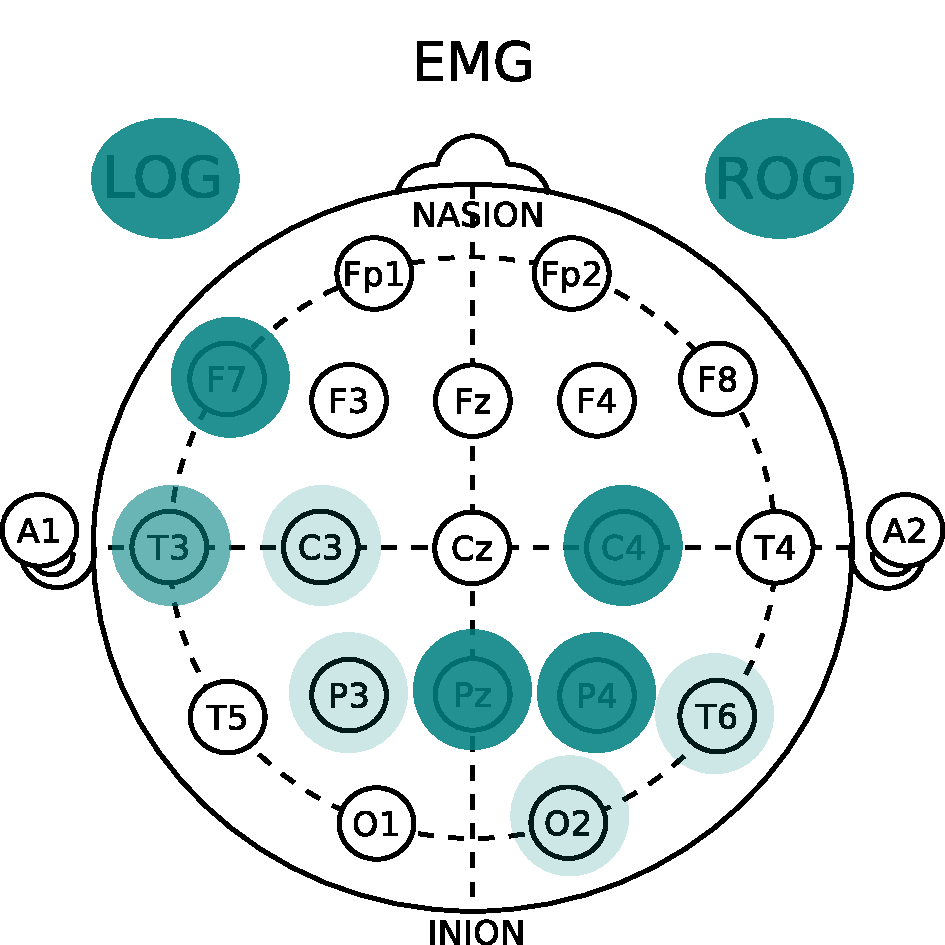
\includegraphics[width=0.17\textwidth]{./img_diagramas/cabecita_JAE.pdf} &
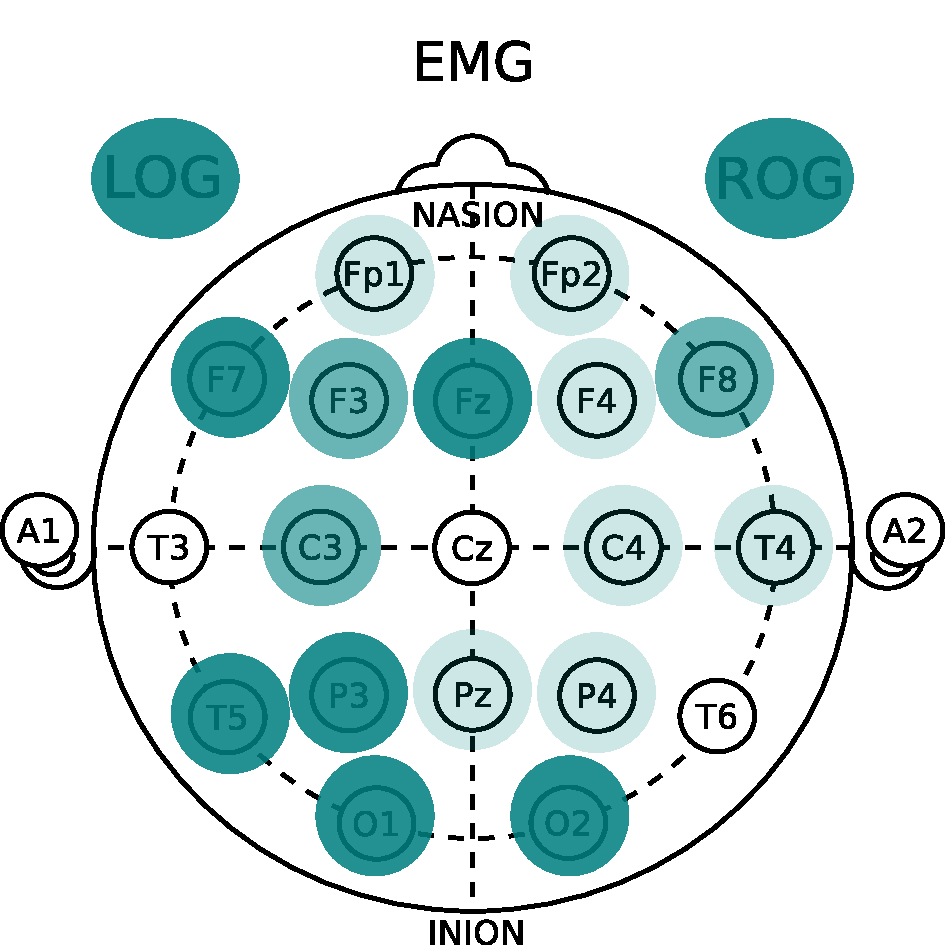
\includegraphics[width=0.17\textwidth]{./img_diagramas/cabecita_GHA.pdf} &
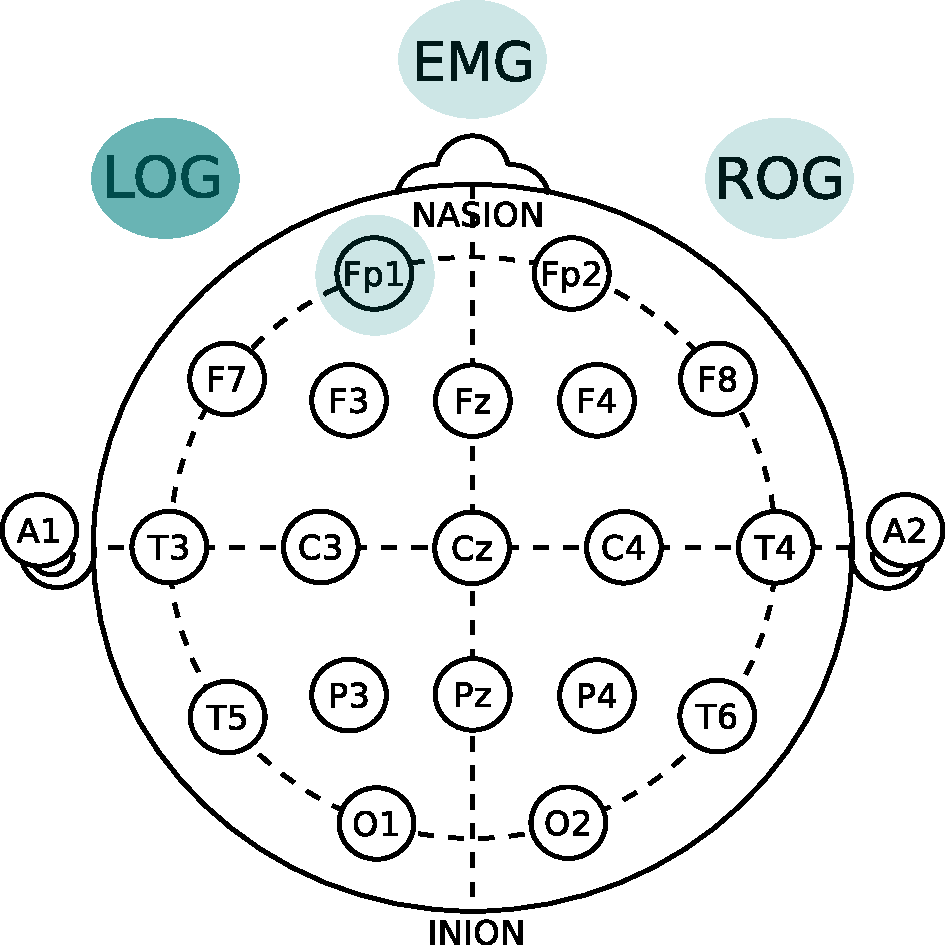
\includegraphics[width=0.17\textwidth]{./img_diagramas/cabecita_MFGR.pdf} \\
VCR & MJH & JAE & GHA & MFGR
\end{tabular}
\\
\begin{tabular}{cccc}
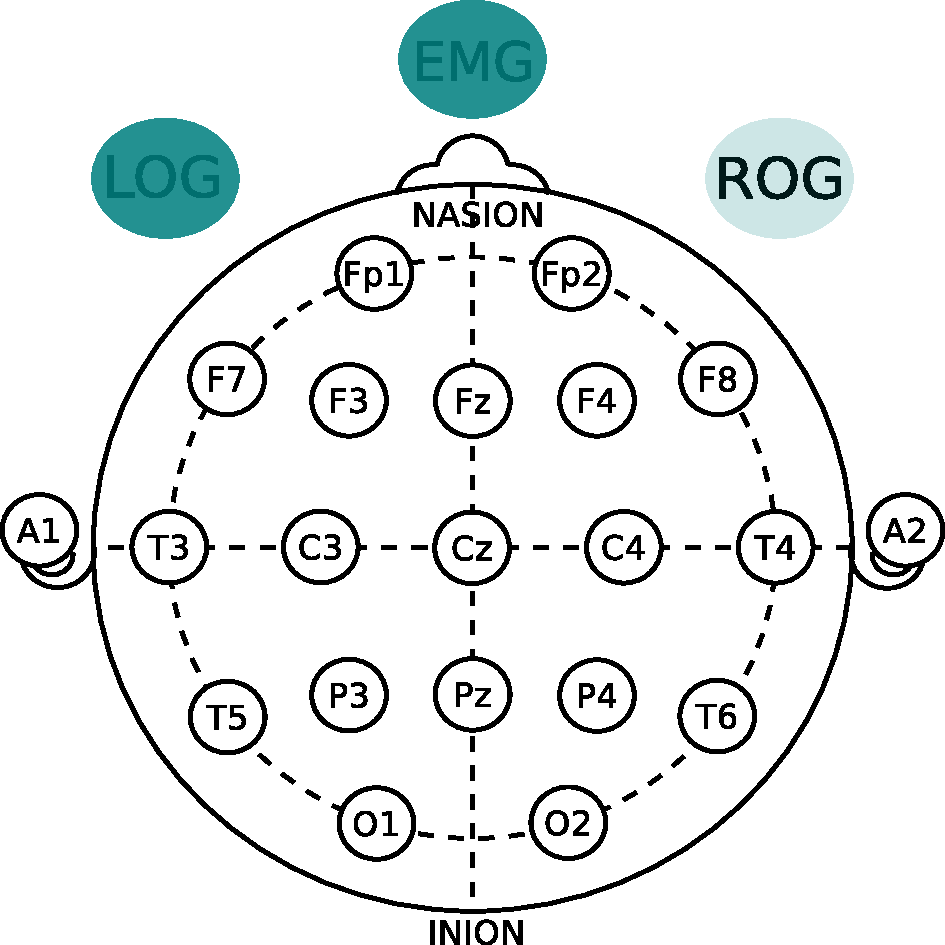
\includegraphics[width=0.17\textwidth]{./img_diagramas/cabecita_CLO.pdf} &
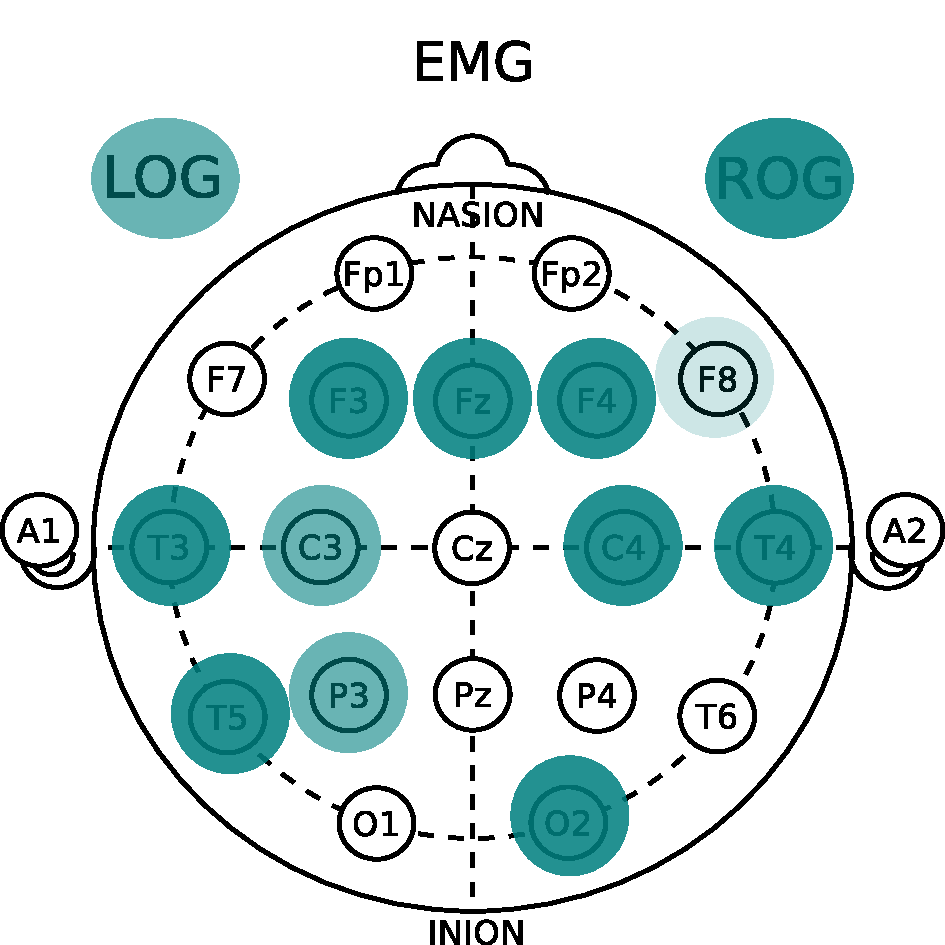
\includegraphics[width=0.17\textwidth]{./img_diagramas/cabecita_RLO.pdf} &
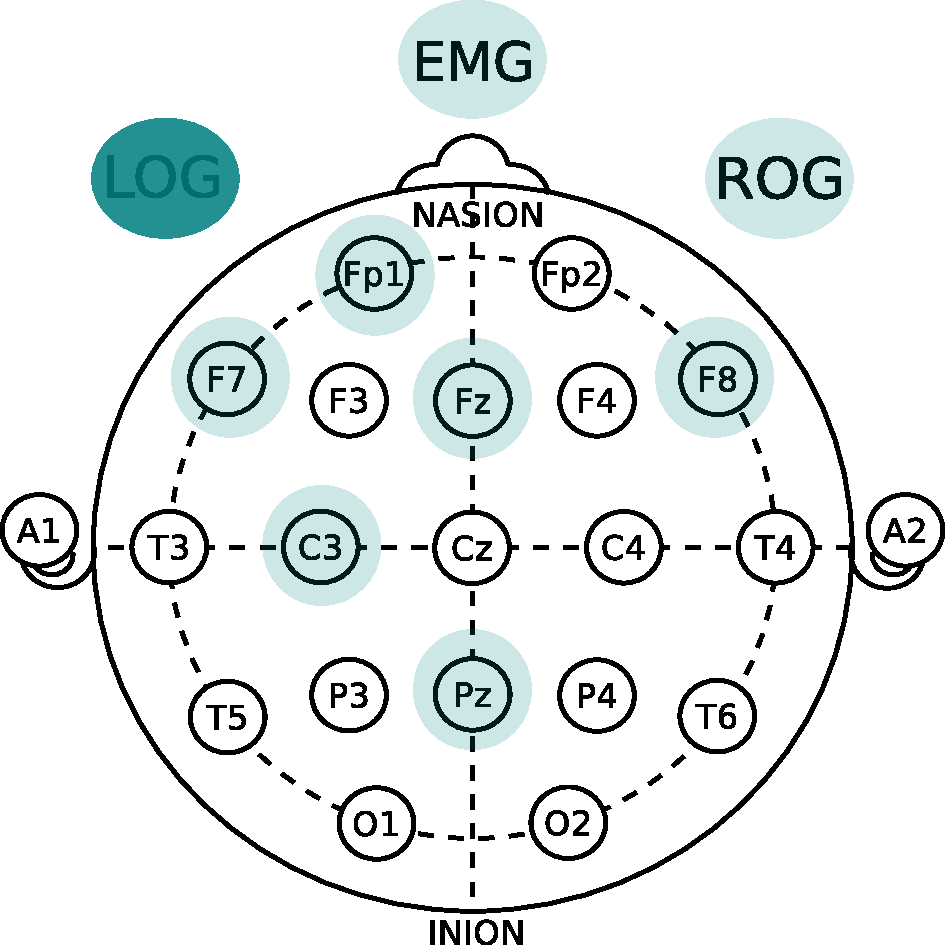
\includegraphics[width=0.17\textwidth]{./img_diagramas/cabecita_RRU.pdf} &
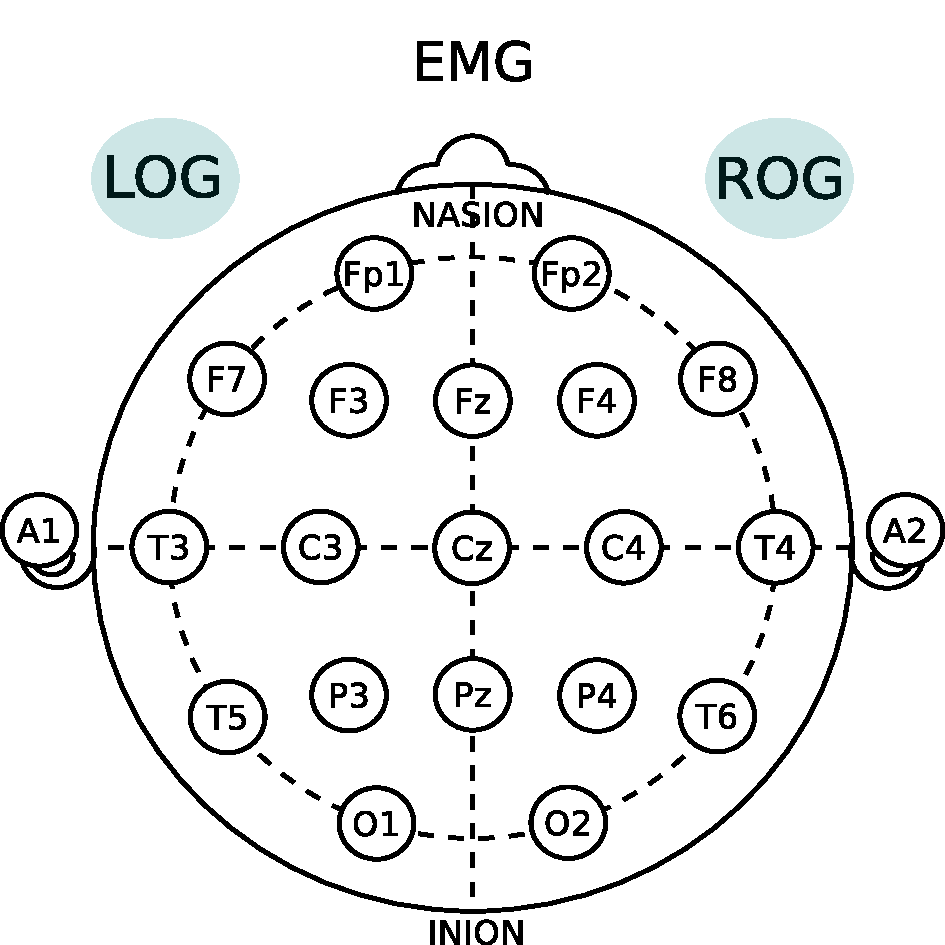
\includegraphics[width=0.17\textwidth]{./img_diagramas/cabecita_JGZ.pdf} \\
CLO & RLO & RRU & JGZ
\end{tabular}
\\
\begin{tabular}{ccc}
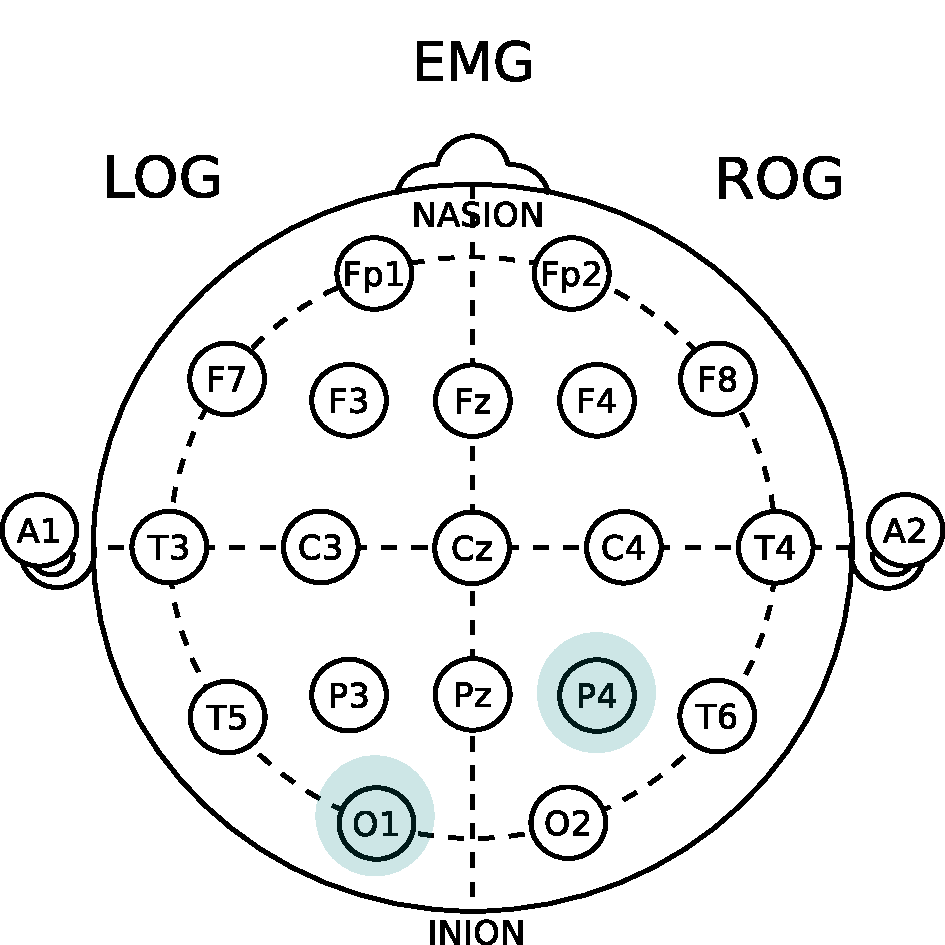
\includegraphics[width=0.17\textwidth]{./img_diagramas/cabecita_FGH.pdf} &
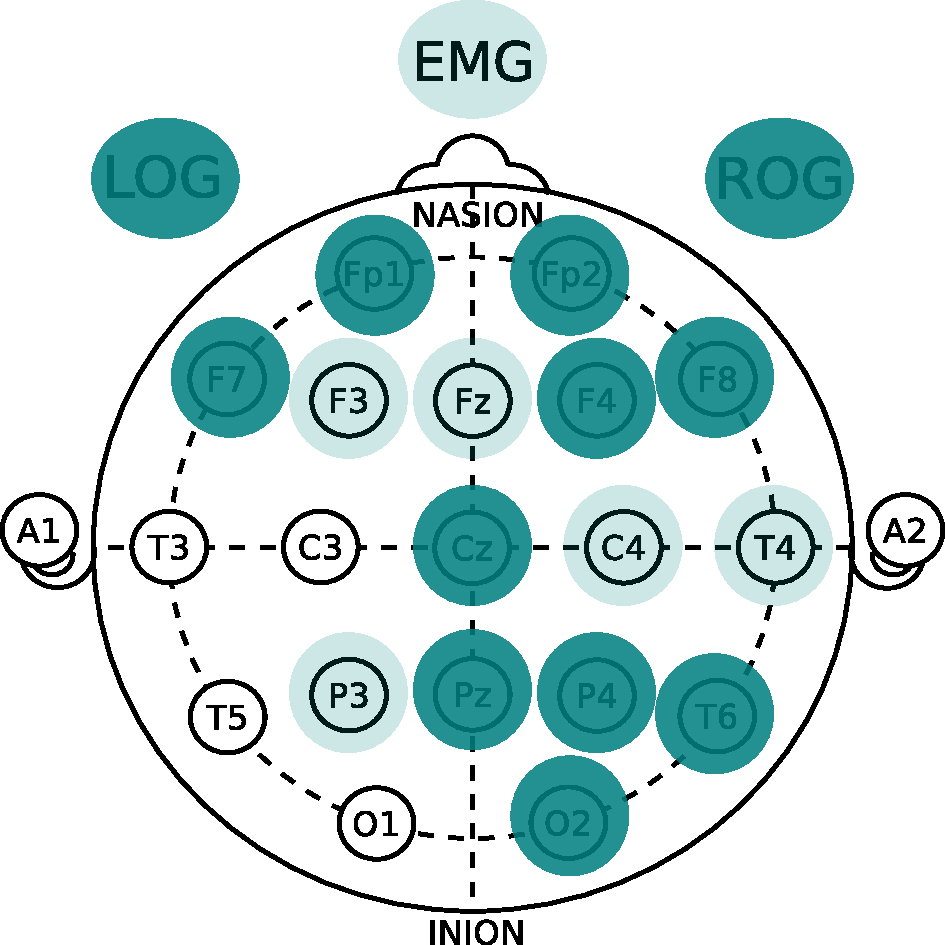
\includegraphics[width=0.17\textwidth]{./img_diagramas/cabecita_MGG.pdf} &
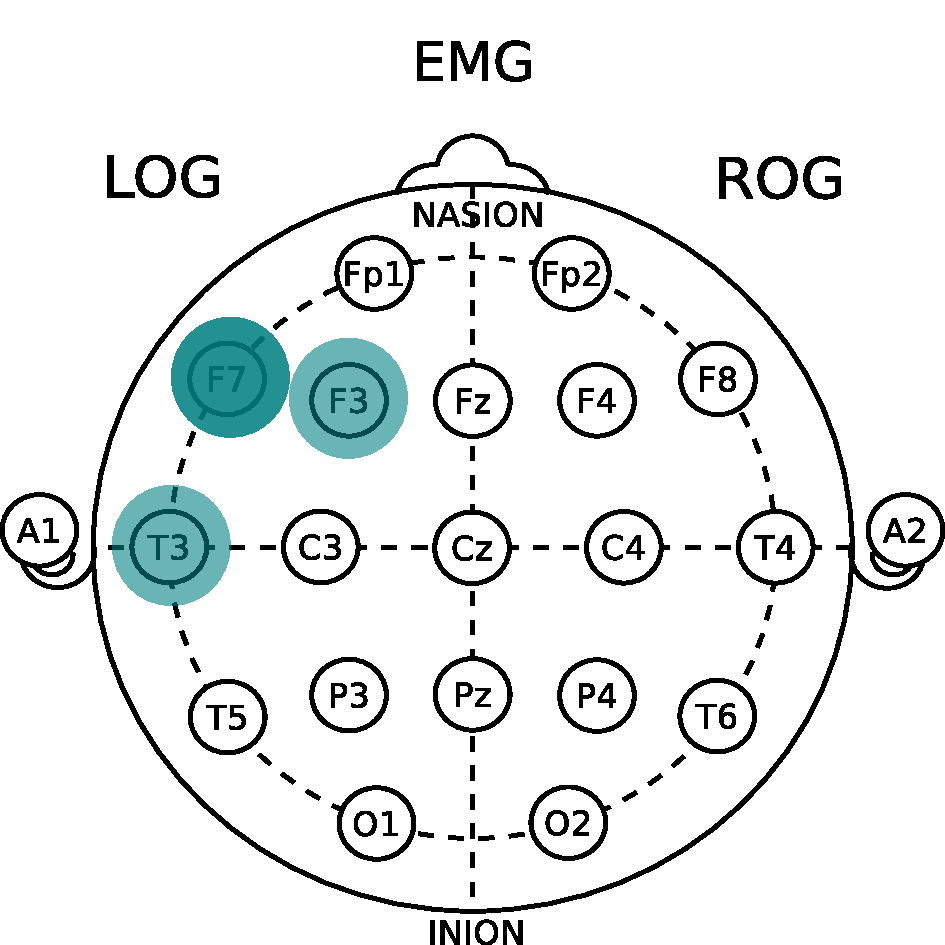
\includegraphics[width=0.17\textwidth]{./img_diagramas/cabecita_EMT.pdf} \\
FGH & MGG & EMT
\end{tabular}
\end{tabular}
\caption{Se muestra esquem\'aticamente en azul las zonas donde se encontraron diferencias 
significativas al comparar las proporciones de \'epocas PE durante sue\~no MOR y NMOR. Esta misma
informaci\'on se muestra en la tabla \ref{comparacion_mor_vs_total} }
\label{cabecitas_munchas}
\end{figure}

Posteriormente se busc\'o una diferencia m\'as directa entre los grupos, comparando grupalmente las 
proporciones de \'epocas PE (en cada canal y durante las diferentes etapas) mediante la prueba U de 
Mann-Whitney\footnote{Implementada en R como la funci\'on \texttt{wilcox.test()}}; no se 
encontraron diferencias significativas para ninguno de los canales. Los resultados se muestran en 
las tablas \ref{gpos_mor}, \ref{gpos_nmor}, \ref{gpos_total}, y para una mejor visualizaci\'on 
\'estos se han graficado en la figura \ref{comparacion_graf}.

\begin{figure}
\centering
\subfloat[Comparaci\'on entre \'epocas MOR (fase R)]{
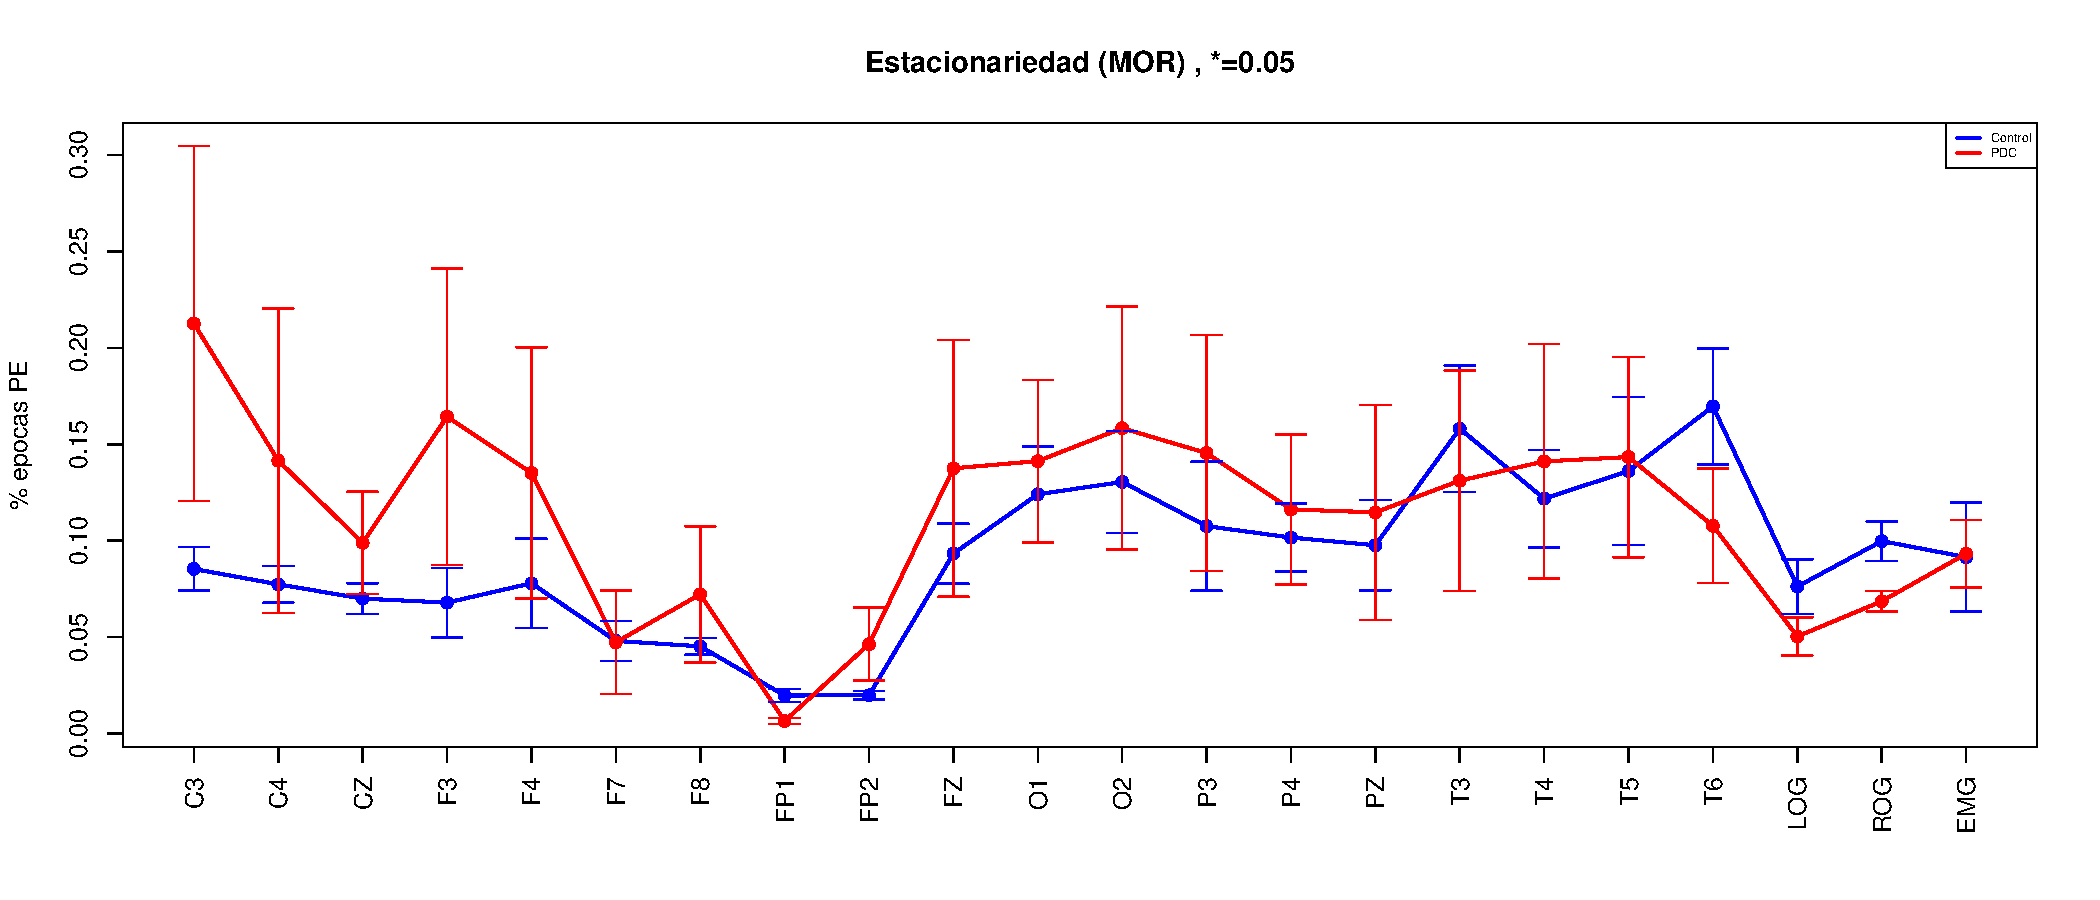
\includegraphics[width=0.95\linewidth]
{./img_ejemplos/Comparacion_gpos_MOR.pdf} 
}\\
\subfloat[Comparaci\'on entre \'epocas no-MOR (fases W y N)]{
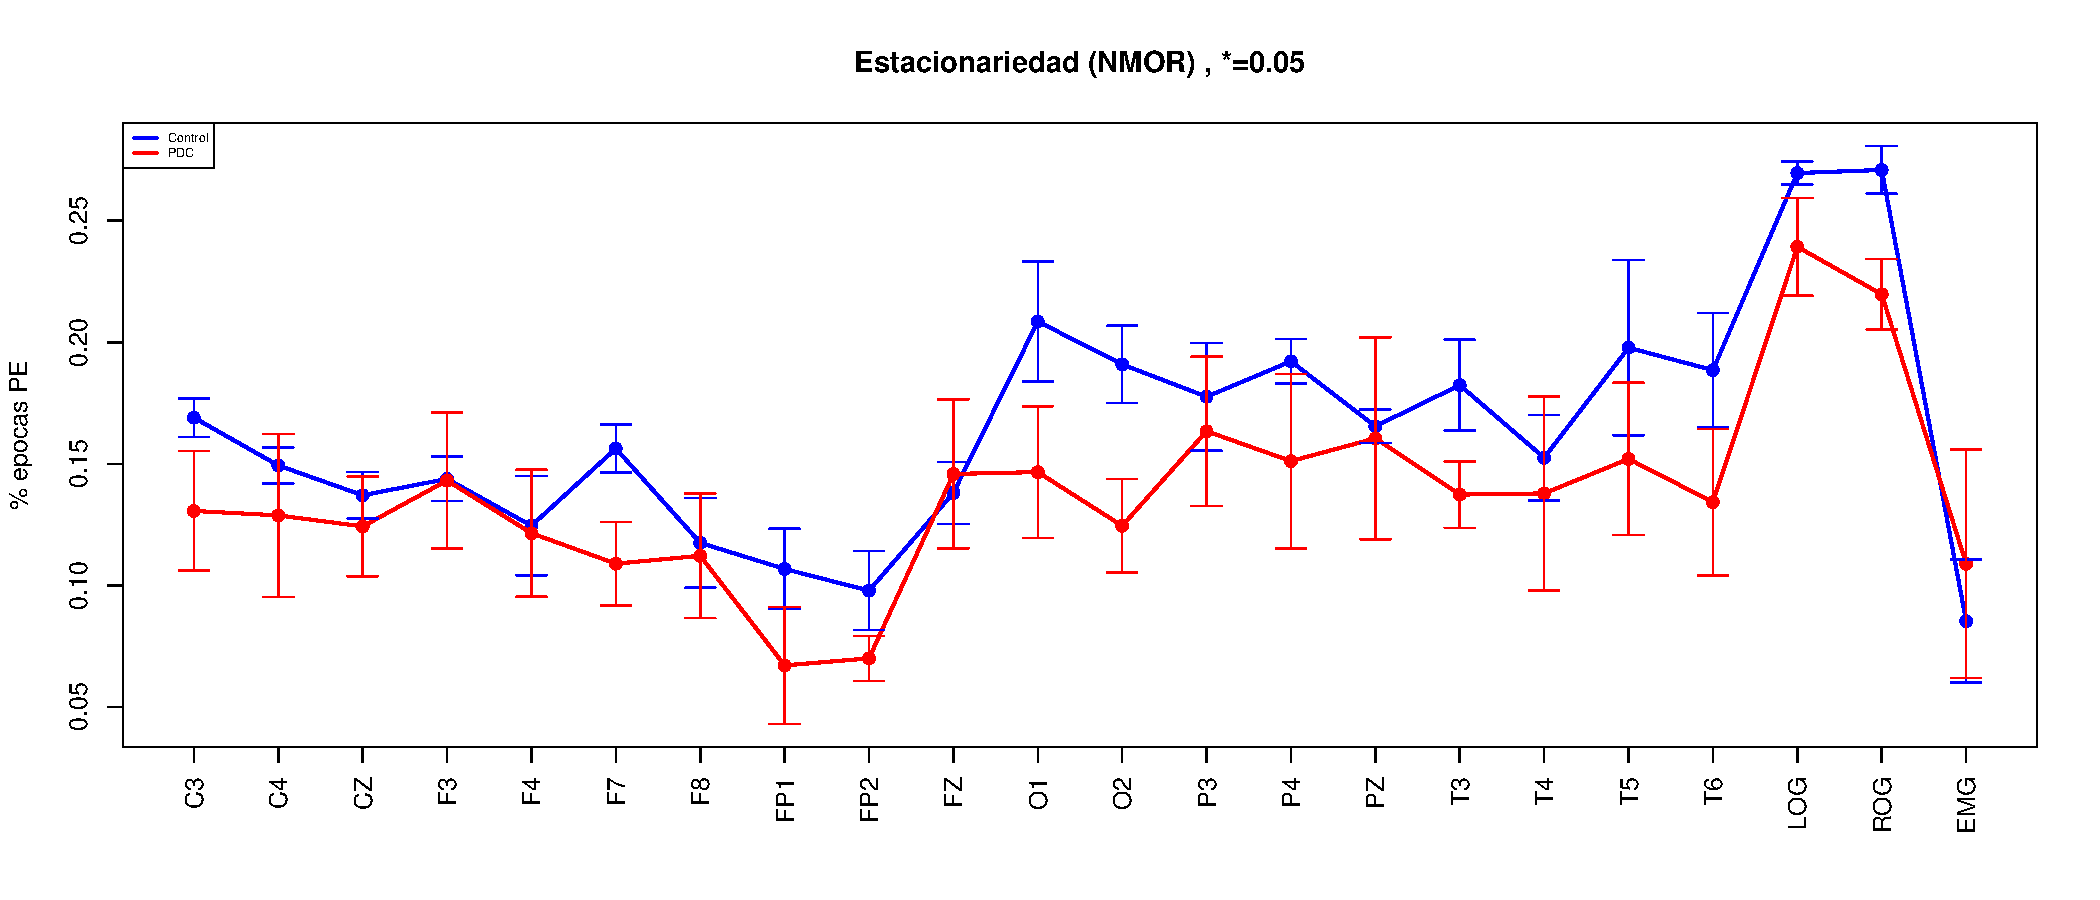
\includegraphics[width=0.95\linewidth]
{./img_ejemplos/Comparacion_gpos_NMOR.pdf} 
}\\
\caption{Comparaci\'on sobre las proporciones de \'epocas PE entre los grupos Control (azul) y PDC 
(rojo), para diferentes etapas de sue\~no (MOR y NMOR). Se grafica el promedio grupal $\pm$ 1 
desviaci\'on est\'andar$^{\nicefrac{3}{2}}$, como visualizaci\'on aproximada de la varianza.}
\label{comparacion_graf}
\end{figure}

Una segunda variaci\'on del primer an\'alisis es considerar grupalmente a los sujetos como 
'unidades' que transitan entre etapas de sue\~no; se comparan grupalmente las proporciones de 
\'epocas PE en cada canal durante sue\~no MOR y NMOR, usando la prueba U de Mann-Whithney; en 
la figura \ref{comparacion_verde} se han representado gr\'aficamente estas diferencias.
Se encontr\'o que hay diferencias significativas ($\alpha<0.1$) para el grupo Control en los 
canales C3, C4, F7, F8, FP1, FP2, O2, P4, LOG y ROG, mientras que en el grupo PDC s\'olo se
observaron diferencias en LOG y ROG.
Descartando los canales LOG y ROG, ya que no son parte del EEG, las diferencias encontradas pueden 
ser relevantes fisiol\'ogicamente, ya que abarcan gran parte de los l\'obulos frontal y parietal, 
y parte de la regi\'on occipital-parietal derecha; en la figura \ref{cabecita} se indican 
esquem\'aticamente estas regiones.

\begin{figure}
\centering
\subfloat[Comparaci\'on para el grupo control]{
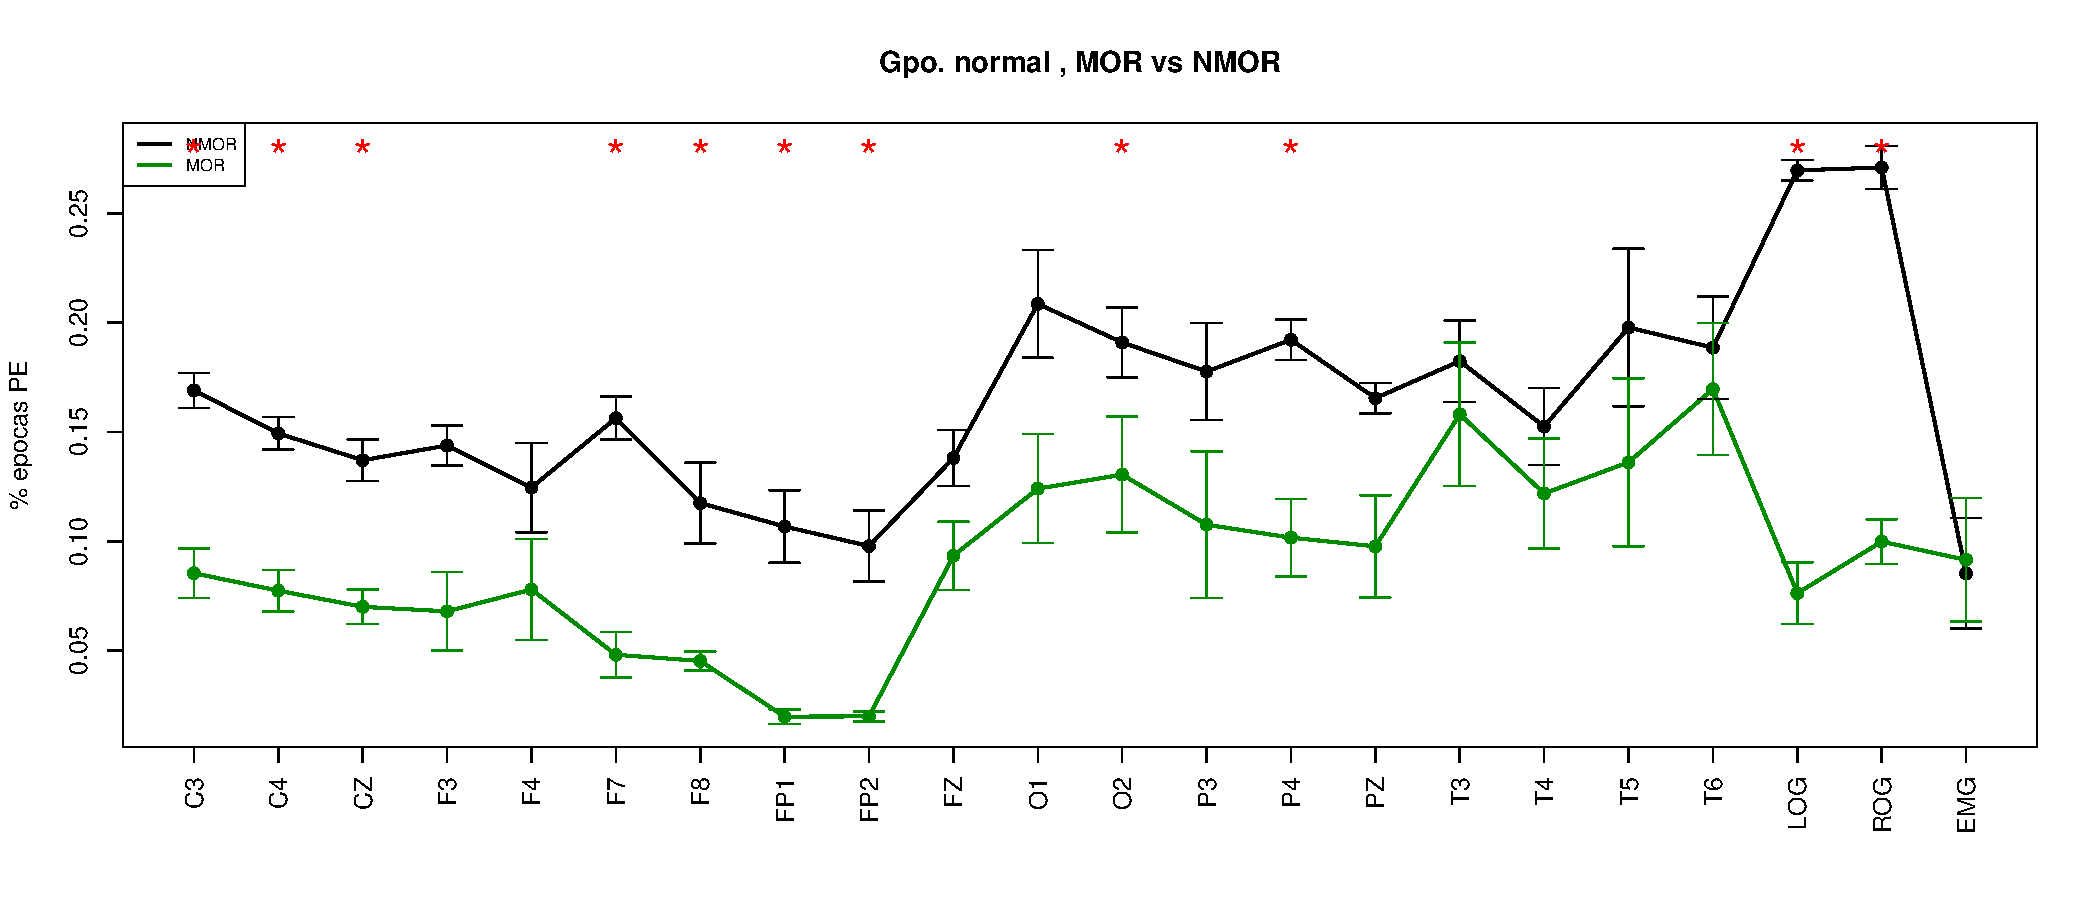
\includegraphics[width=0.95\linewidth]
{./img_ejemplos/comp_etapas_gpos_NORMALMOR_vs_NMOR.pdf} 
}\\
\subfloat[Comparaci\'on para el grupo PDC]{
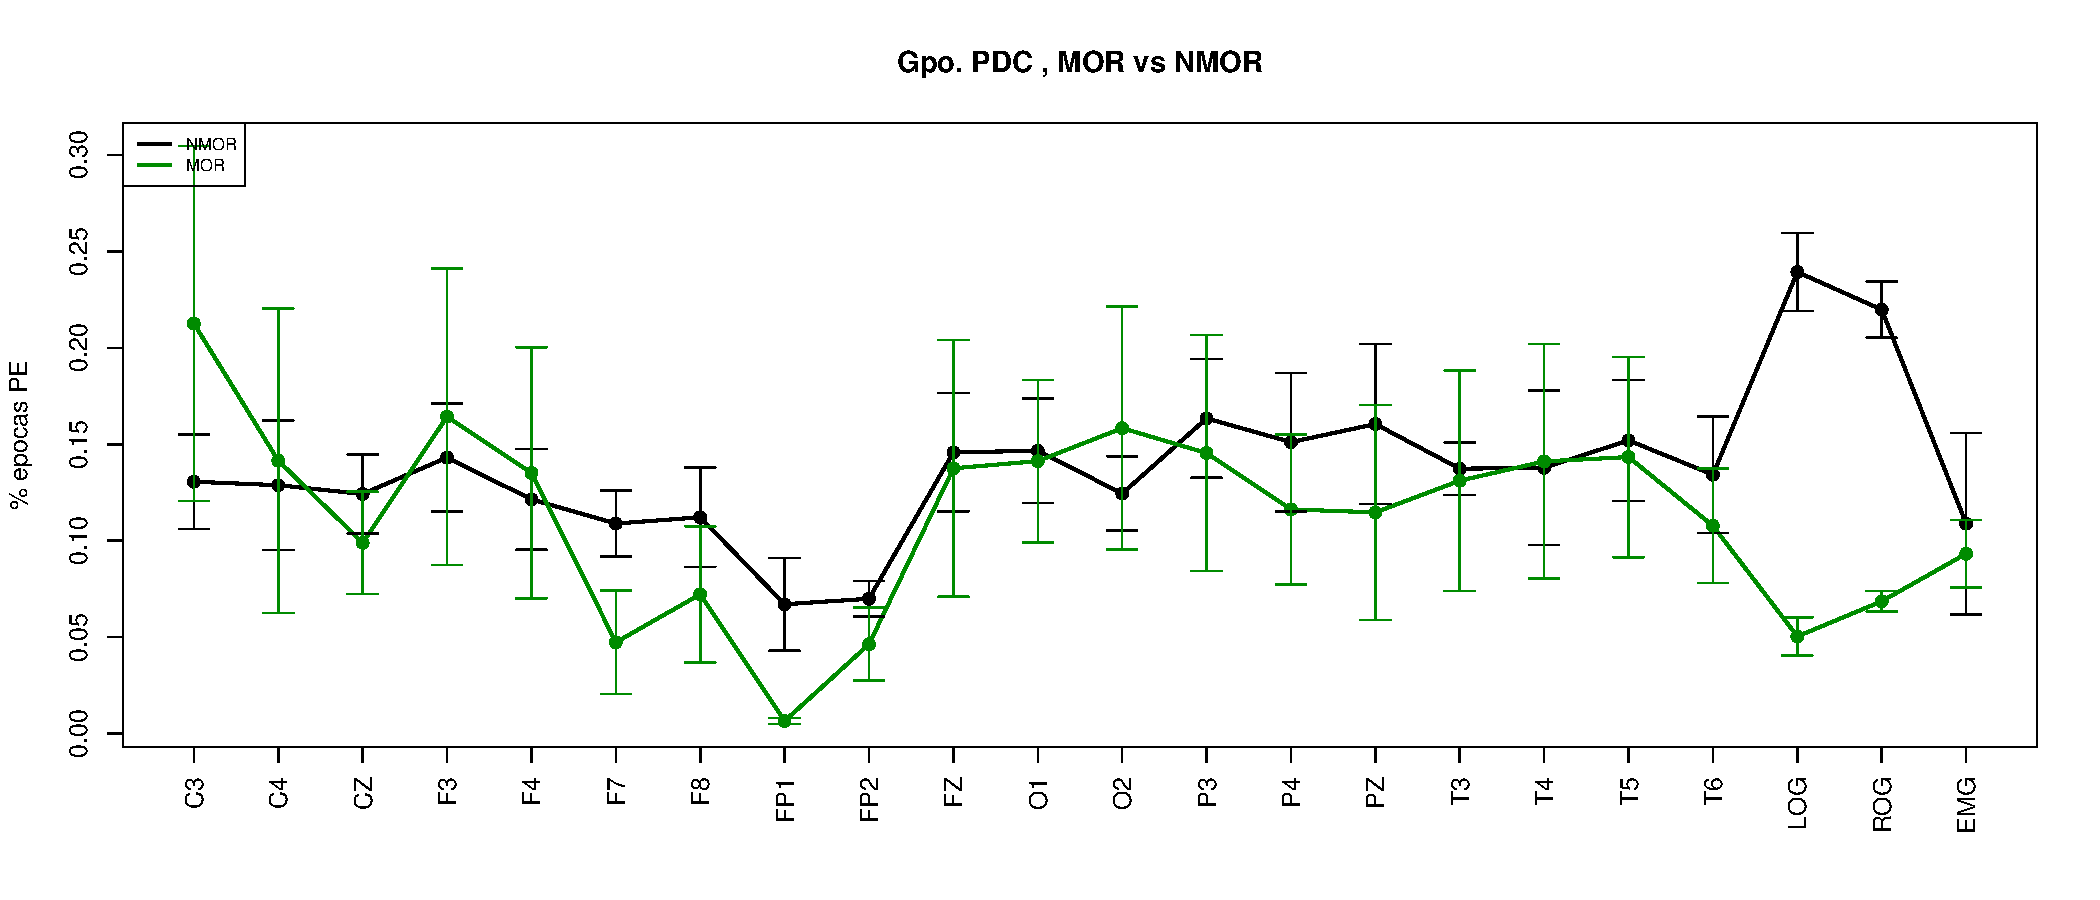
\includegraphics[width=0.95\linewidth]
{./img_ejemplos/comp_etapas_gpos_PDCMOR_vs_NMOR.pdf} 
}
\caption{Comparaci\'on sobre las proporciones de \'epocas PE entre las etapas de sue\~no MOR 
(verde) y NMOR (negro), para ambos grupos por separado. Se han graficado las proporciones de PE en 
todos los sujetos de cada grupo, para todo el sue\~no y la etapa MOR.
Se grafica el promedio grupal $\pm$ 1 desviaci\'on est\'andar$^{\nicefrac{3}{2}}$, como 
visualizaci\'on aproximada de la varianza.}
\label{comparacion_verde}
\end{figure}

\begin{figure}
\centering
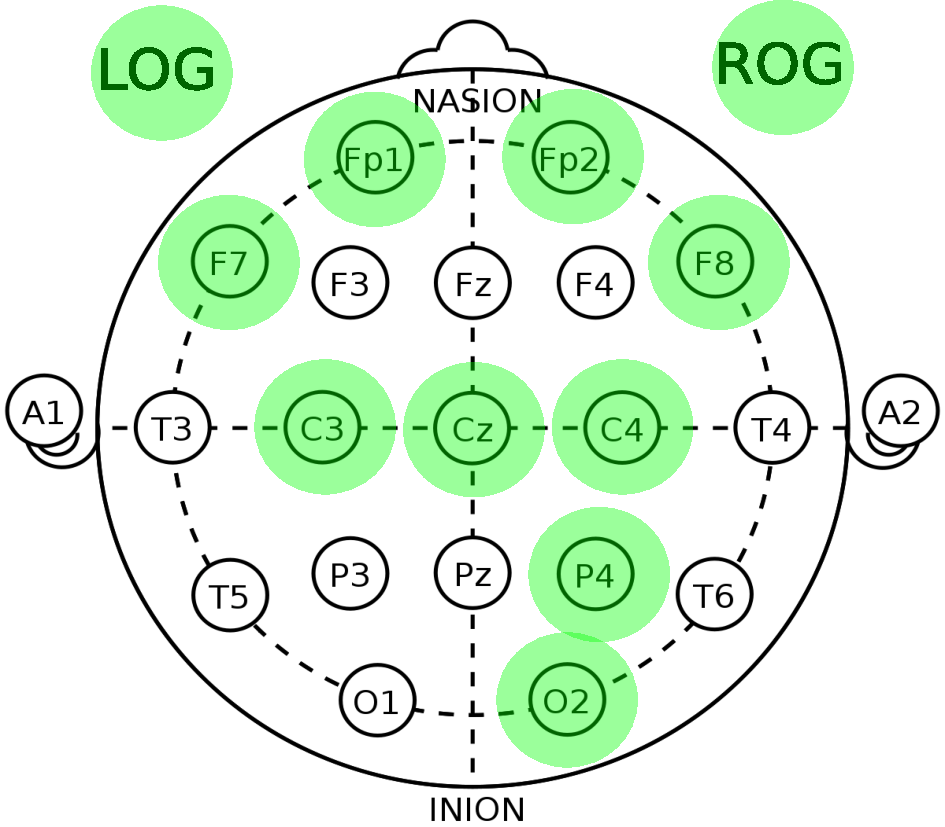
\includegraphics[width=0.4\linewidth]
{./img_diagramas/cabecita.pdf} 
\caption{Representaci\'on esquem\'atica de los sitios donde se encontraron diferencias 
significativas en la comparaci\'on entre el porcentaje de \'epocas PE durante sue\~no MOR y NMOR, 
para el grupo Control (ver texto)}
\label{cabecita}
\end{figure}

%%%%%%%%%%%%%%%%%%%%%%%%%%%%%%%%%%%%%%%%%%%%%%%%%%%%%%%%%%%%%%%%%%%%%%%%%%%%%%%%%%%%%%%%%%%%%%%%%%%
%%%%%%%%%%%%%%%%%%%%%%%%%%%%%%%%%%%%%%%%%%%%%%%%%%%%%%%%%%%%%%%%%%%%%%%%%%%%%%%%%%%%%%%%%%%%%%%%%%%

\section{Patrones visuales}

Como un an\'alisis exploratorio, buscando explicar la variabilidad entre los resultados, se 
graficaron los resultados obtenidos con la prueba PSR de la siguiente manera: se colocan en 
l\'inea horizontal una serie de cuadros, uno por cada \'epoca analizada seg\'un fue clasificada 
(blanco: PE, negro: no-estacionario), y posteriormente se juntaron verticalmente las l\'ineas
correspondientes a los diferentes canales; en la figura \ref{ejemplo_graf} se muestra un ejemplo de
ello, mientras que en el anexo se muestran los gr\'aficos construidos para cada uno de los sujetos. 

Al construir estos gr\'aficos, se hacen presentes 'bloques' de \'epocas que en su mayor\'ia son
PE --similarmente con \'epocas no-estacionarias. Ha parecido conveniente reportar este hallazgo
ya que los patrones son consistentes en todos los sujetos, y porque parece que estos 'bloques'
aparecen asociados al sue\~no MOR en cierto orden (ilustrado en la figura \ref{patroncito}):
\begin{itemize}
\item Bloque abundante en \'epocas PE, visualmente oscuro
\item Bloque abundante en \'epocas no-estacionarias, visualmente claro
\item Secci\'on que contiene el sue\~no MOR, los canales LOG y ROG muestran son visualmente m\'as
abundante en \'epocas no-estacionarias en esta zona del tiempo
\end{itemize}

\begin{figure}
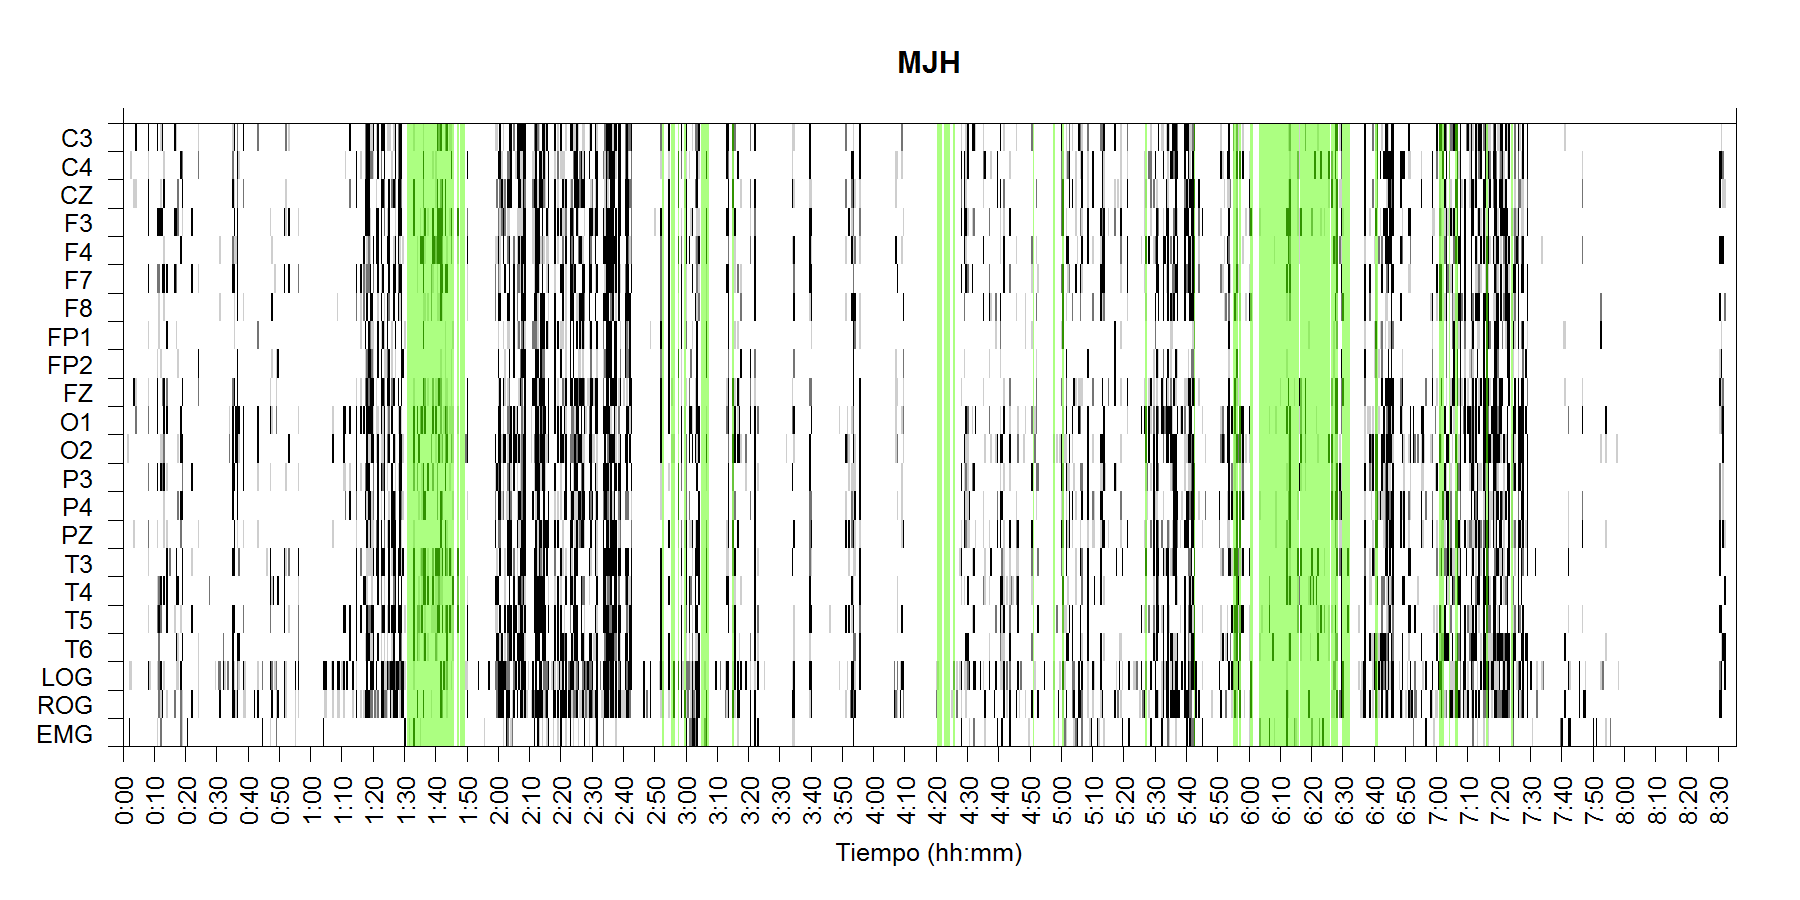
\includegraphics[width=\textwidth]
{./img_ejemplos/MJNNVIGILOS_est.png}
\caption{Disposici\'on gr\'afica para los resultados de la prueba PSR en el sujeto MJH. Se han 
resaltado con color verde las \'epocas clasificadas como de sue\~no MOR.}
\label{ejemplo_graf}
\end{figure}

\begin{figure}
\begin{tabular}{c}
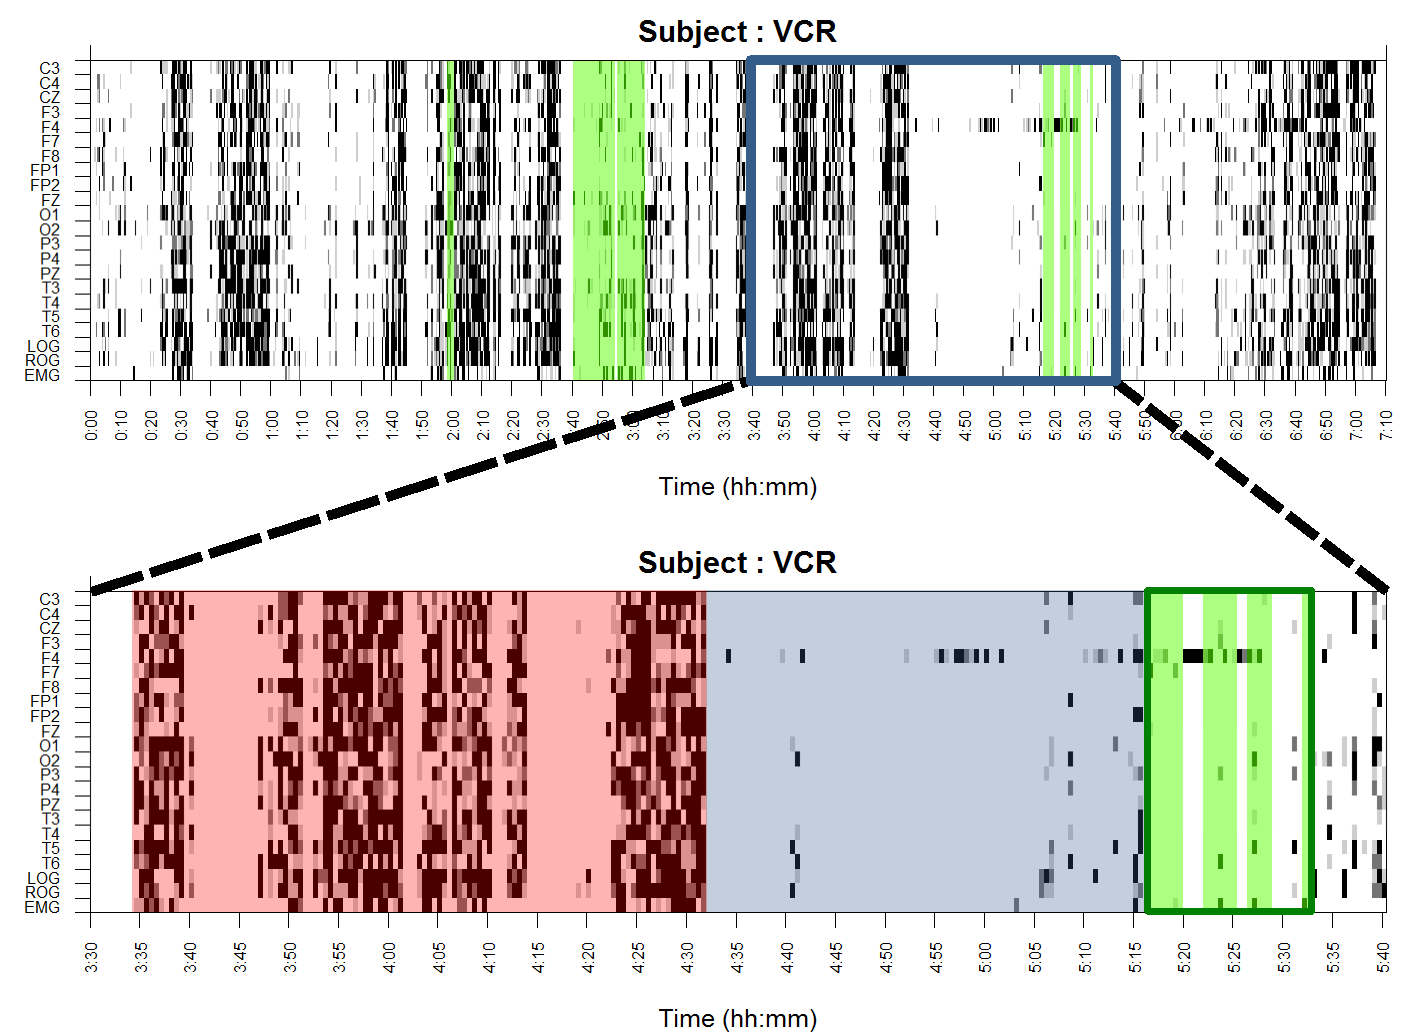
\includegraphics[width=0.3\textwidth]
{./img_ejemplos/zoom_VCR.pdf}
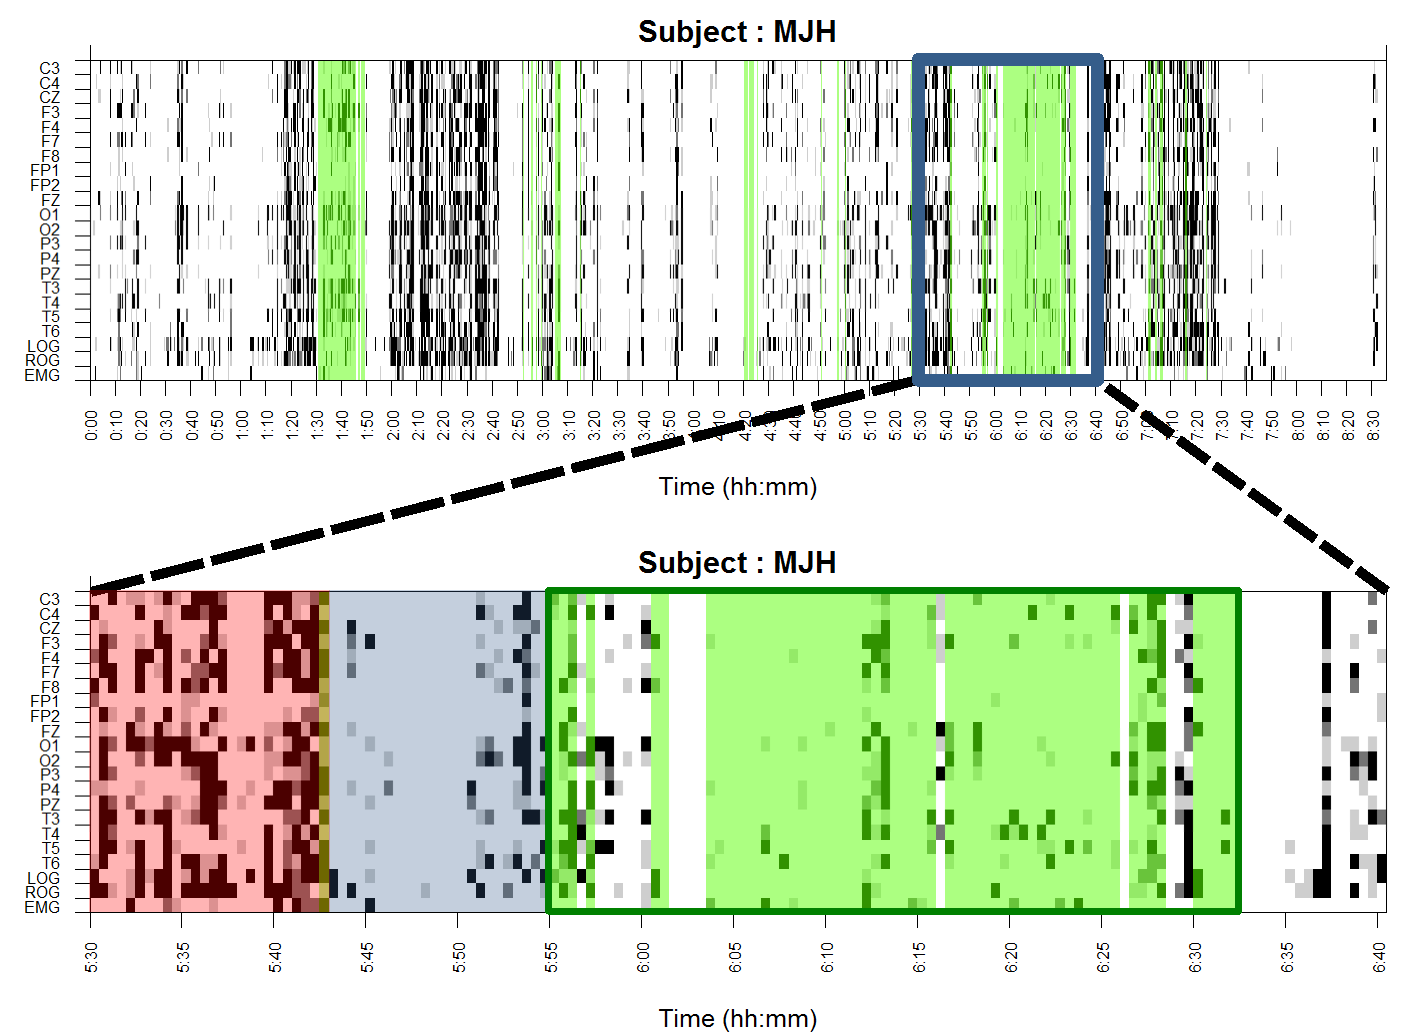
\includegraphics[width=0.3\textwidth]
{./img_ejemplos/zoom_MJH.pdf}
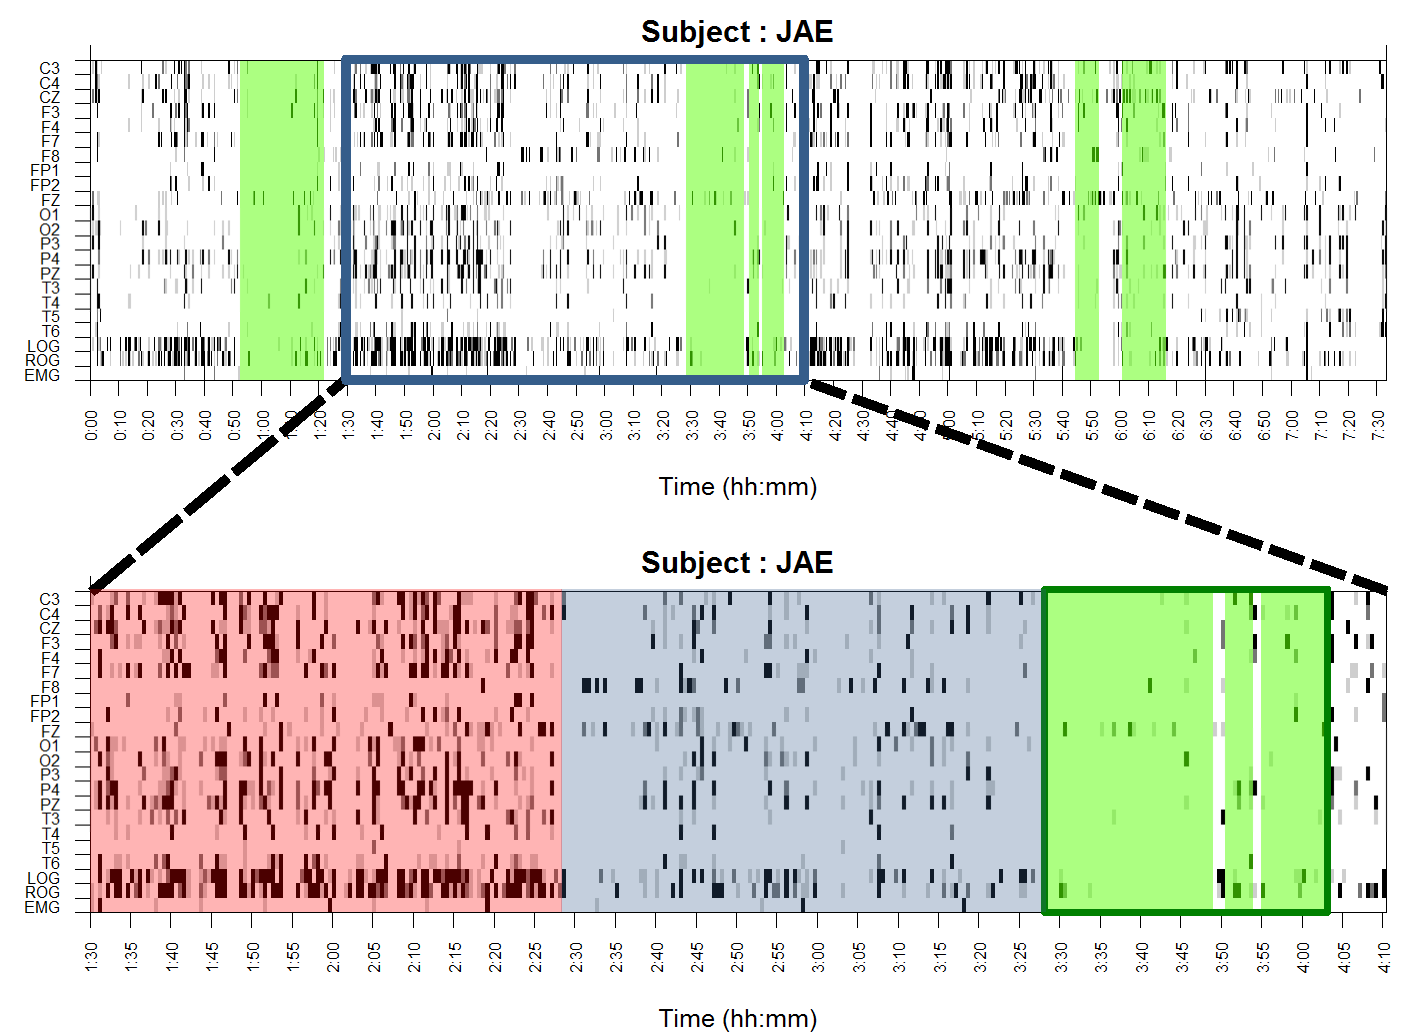
\includegraphics[width=0.3\textwidth]
{./img_ejemplos/zoom_JAE.pdf}
\\
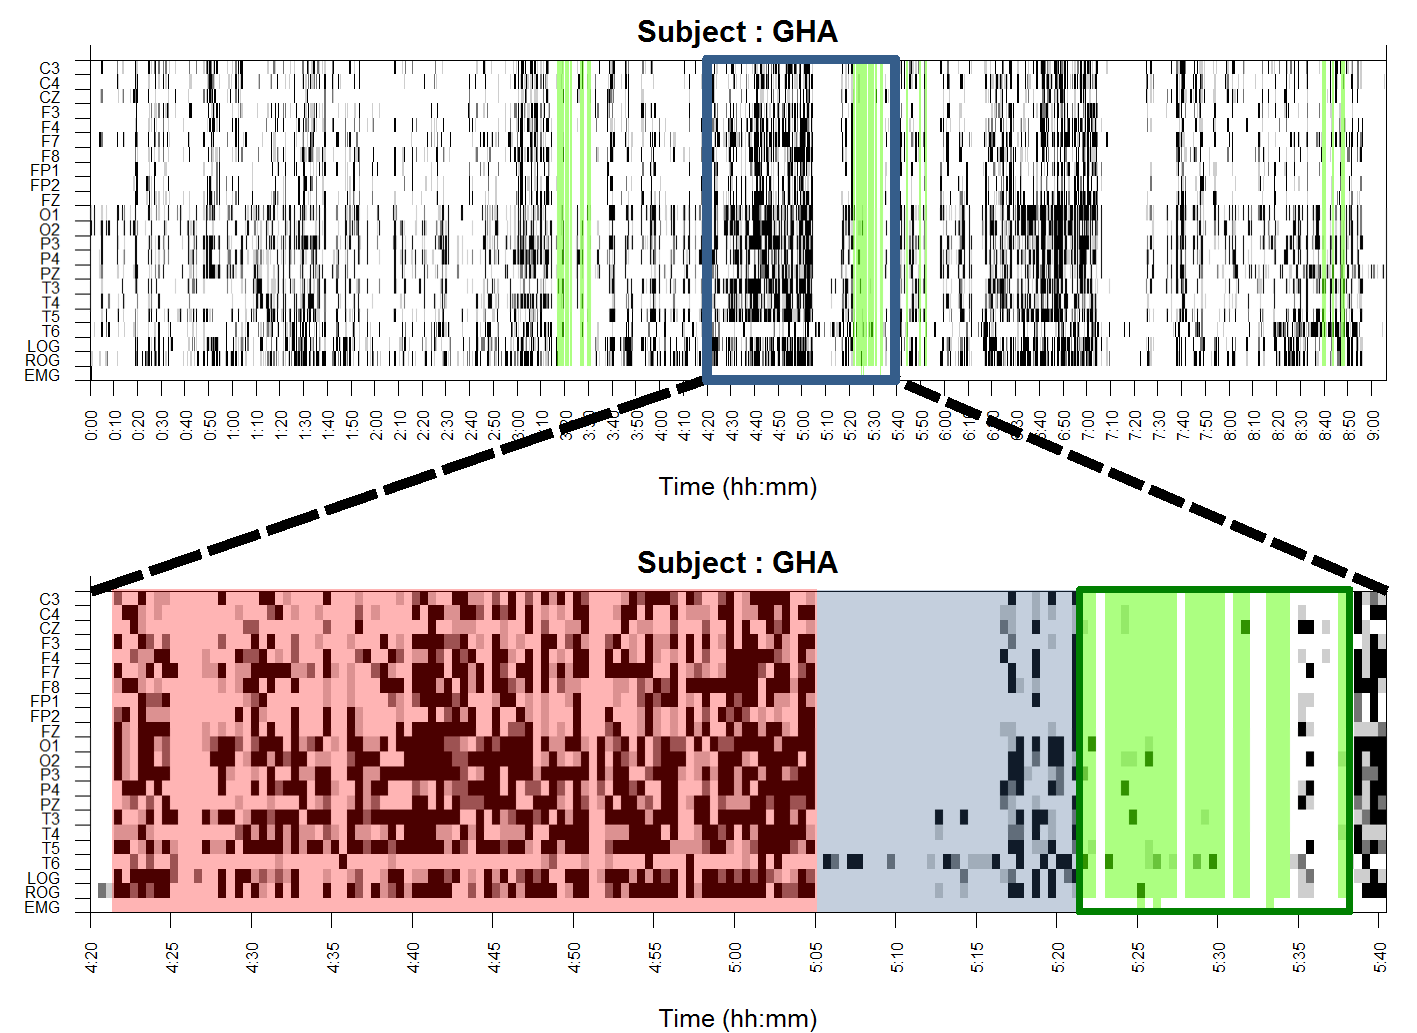
\includegraphics[width=0.3\textwidth]
{./img_ejemplos/zoom_GHA.pdf}
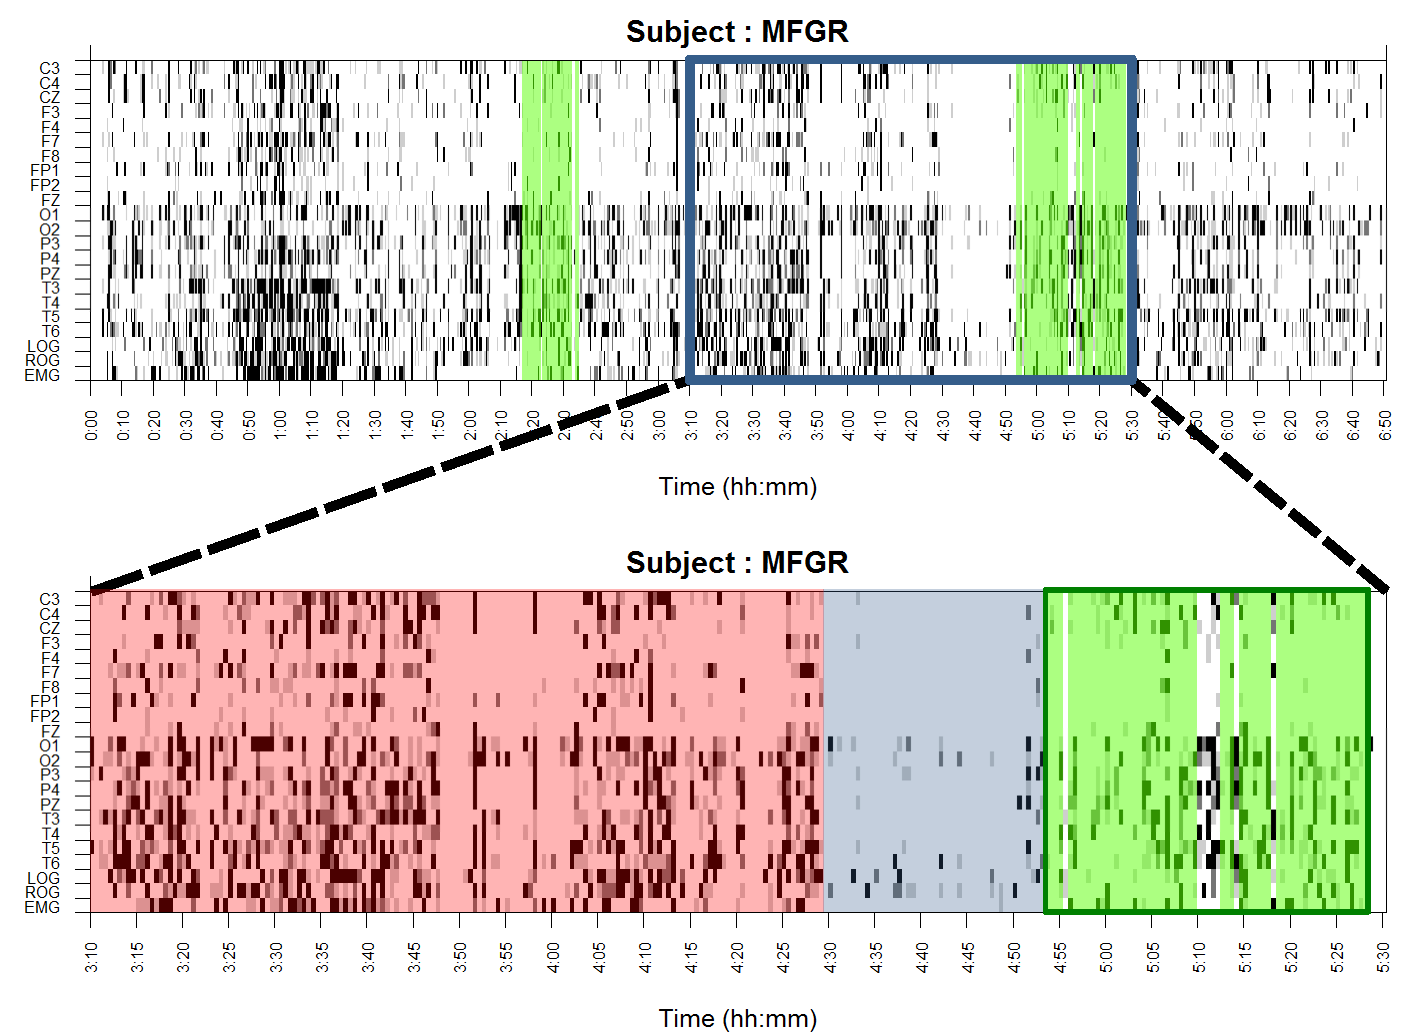
\includegraphics[width=0.3\textwidth]
{./img_ejemplos/zoom_MFGR.pdf}
\end{tabular}
\caption{Ejemplos de los patrones visuales que, se propone, est\'a asociado con la aparici\'on del
sue\~no MOR: un bloque de \'epocas PE (rojo), un bloque de \'epocas no-estacionarias (azul) y un 
bloque que contiene al sue\~no MOR. En este ejemplo se ilustra uno de estos patrones por cada
uno de los sujetos del grupo Control.}
\label{patroncito}
\end{figure}

%%%%%%%%%%%%%%%%%%%%%%%%%%%%%%%%%%%%%%%%%%%%%%%%%%%%%%%%%%%%%%%%%%%%%%%%%%%%%%%%%%%%%%%%%%%%%%%%%%%
%%%%%%%%%%%%%%%%%%%%%%%%%%%%%%%%%%%%%%%%%%%%%%%%%%%%%%%%%%%%%%%%%%%%%%%%%%%%%%%%%%%%%%%%%%%%%%%%%%%
%%%%%%%%%%%%%%%%%%%%%%%%%%%%%%%%%%%%%%%%%%%%%%%%%%%%%%%%%%%%%%%%%%%%%%%%%%%%%%%%%%%%%%%%%%%%%%%%%%%
%%%%%%%%%%%%%%%%%%%%%%%%%%%%%%%%%%%%%%%%%%%%%%%%%%%%%%%%%%%%%%%%%%%%%%%%%%%%%%%%%%%%%%%%%%%%%%%%%%%

\section{Discusi\'on}

Como se mencion\'o anteriormente, este trabajo parte del supuesto en que los sujetos con PDC 
presentan con mayor probabilidad estacionariedad d\'ebil en sus registros de EEG.
Se ha aportado evidencia para afirmar que, al comparar sujetos del grupo Control y con PDC, no hay 
cambios significativos en la porci\'on de tiempo durante la cual el registro de PSG se comporta 
como d\'ebilmente estacionario. 
Esto puede interpretarse como que, quiz\'a, los mecanismos afectados durante el PDC no provocan que 
la se\~nal se vuelva m\'as 'simple' (en el sentido de ser estacionaria).

Cabe un comentario sobre c\'omo la evidencia presentada exhibe al PSG como un conjunto de se\~nales 
no-estacionarias durante la mayor parte del sue\~no, como se suele suponer en se\~nales de origen 
biol\'ogico; entonces, no es adecuado analizar este tipo de se\~nales con m\'etodos que supongan 
estacionariedad, como la estimaci\'on del espectro de potencias usando el periodograma 'cl\'asico'. 

%%%%%%%%%%%%%%%%%%%%%%%%%%%%%%%%%%%%%%%%%%%%%%%%%%%%%%%%%%%%%%%%%%%%%%%%%%%%%%%%%%%%%%%%%%%%%%%%%%%
%%%%%%%%%%%%%%%%%%%%%%%%%%%%%%%%%%%%%%%%%%%%%%%%%%%%%%%%%%%%%%%%%%%%%%%%%%%%%%%%%%%%%%%%%%%%%%%%%%%

\subsection{Sobre los sujetos excluidos}

Durante el trabajo se mencionan tres sujetos (FGH, MGG, EMT) cuyos registros de PSG fueron 
analizados pero que no son considerados estad\'isticamente; cada uno de ellos fue excluido, por 
diversos motivos, del trabajo por V\'azquez Tagle y colaboradores \cite{VazquezTagle16}, pero 
dieron su consentimiento informado para el registro de PSG, debido a lo cual analiz\'o el efecto de 
su inclusi\'on dentro de los an\'alisis.
Destaca el sujeto FGH, quien padece de par\'alisis facial, cataratas, y problemas no especificados 
en hipotiroides y columna; seg\'un se reporta, el sujeto no inform\'o de estos \'ultimos 
padecimientos sino hasta despu\'es del registro de PSG, por lo que su exclusi\'on se efectu\'o a 
posteriori.

Un vistazo a los registros 'inusuales' de FGH (figura\ref{FGH_psg}, comparar con 
\ref{ejemplos_mor}) pudiera haber advertido que en el registro no hay actividad cerebral en los 
canales correspondientes a la regi\'on izquierda (aquella con par\'alisis) sino ruido amplificado 
del polisomn\'ografo.
Dentro del marco de este trabajo, destacan las proporciones inusuales de \'epocas PE (cercanas a 1 
o 0) para este sujeto en los canales F4, F7, F8, FP1, FP2, FZ, tanto en sue\~no MOR como NMOR; 
usando la representaci\'on gr\'afica para FGH, es visible una inusual ausencia total de 
estacionariedad en tales canales (figura \ref{FGH_especial}, comparar con \ref{ejemplo_graf}). 
Si bien esta metodolog\'ia no se dise\~n\'o para tal fin, a\'un as\'i se pudo detectar la falta de 
actividad cerebral.

\begin{figure}
\centering
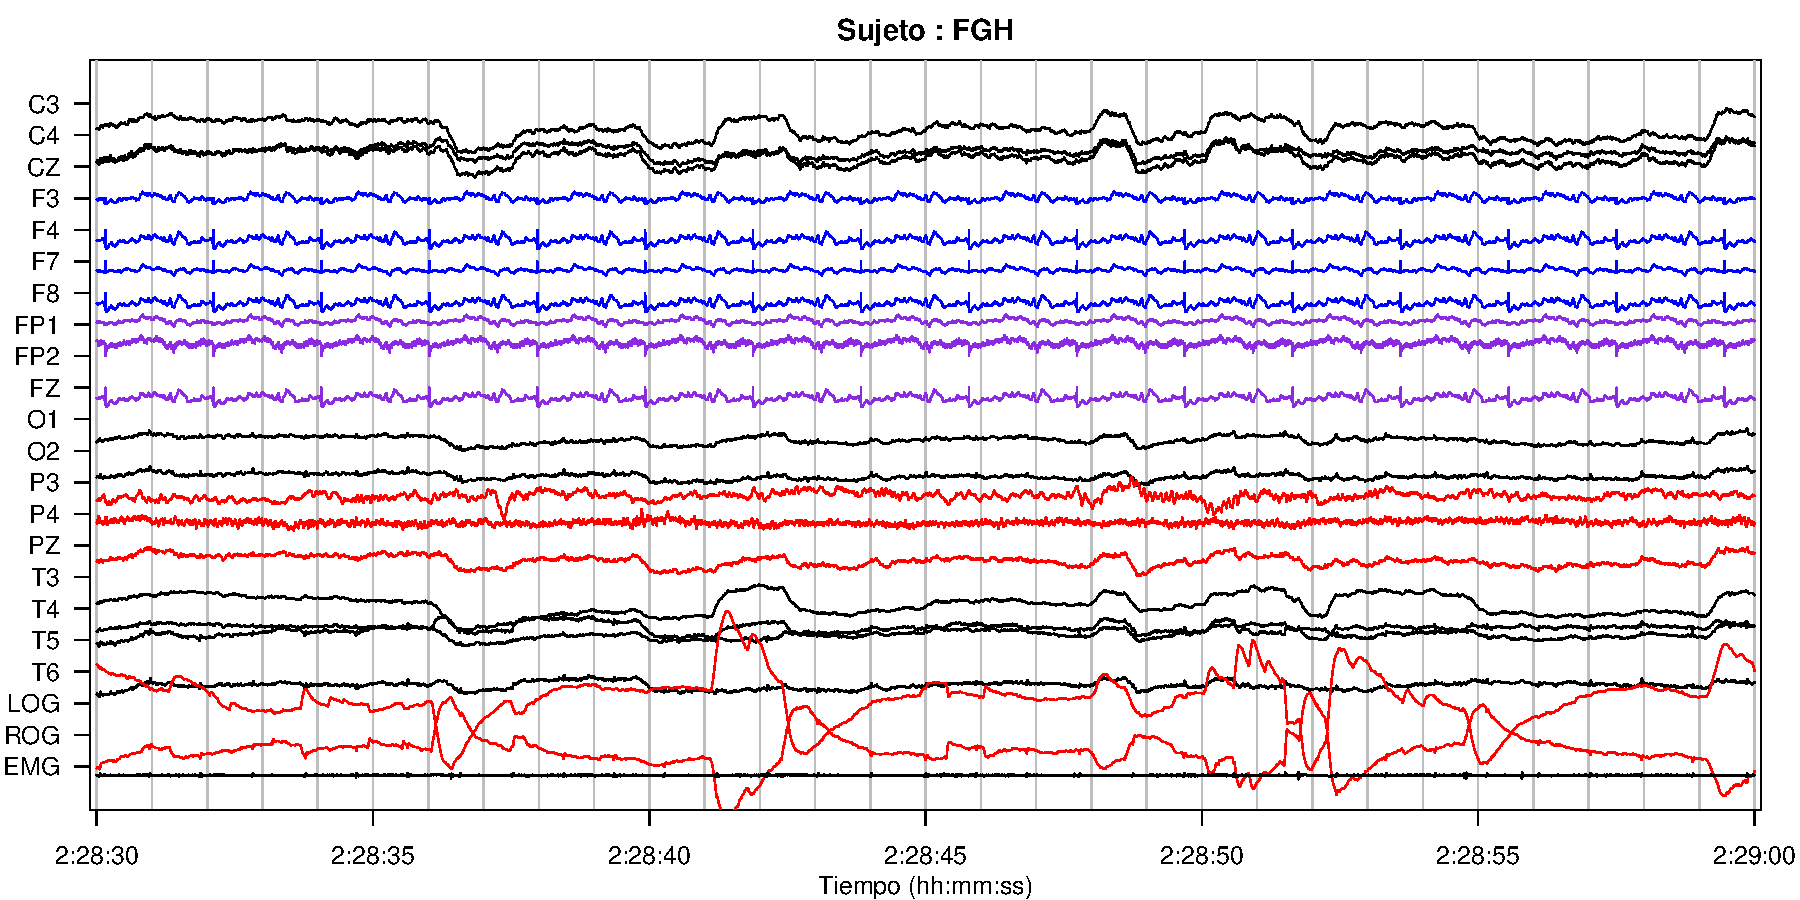
\includegraphics[width=0.95\linewidth]
{./img_ejemplos/FGH_297_PDG_lucirse_PSG.pdf} 
\caption{Una \'epoca t\'ipica del registro PSG para el sujeto FGH durante sue\~no MOR. N\'otense 
los patrones peri\'odicos en los canales correspondientes a la regi\'on frontal, que no 
corresponden a la actividad cerebral usual.}
\label{FGH_psg}
\end{figure}

\begin{figure}
\centering
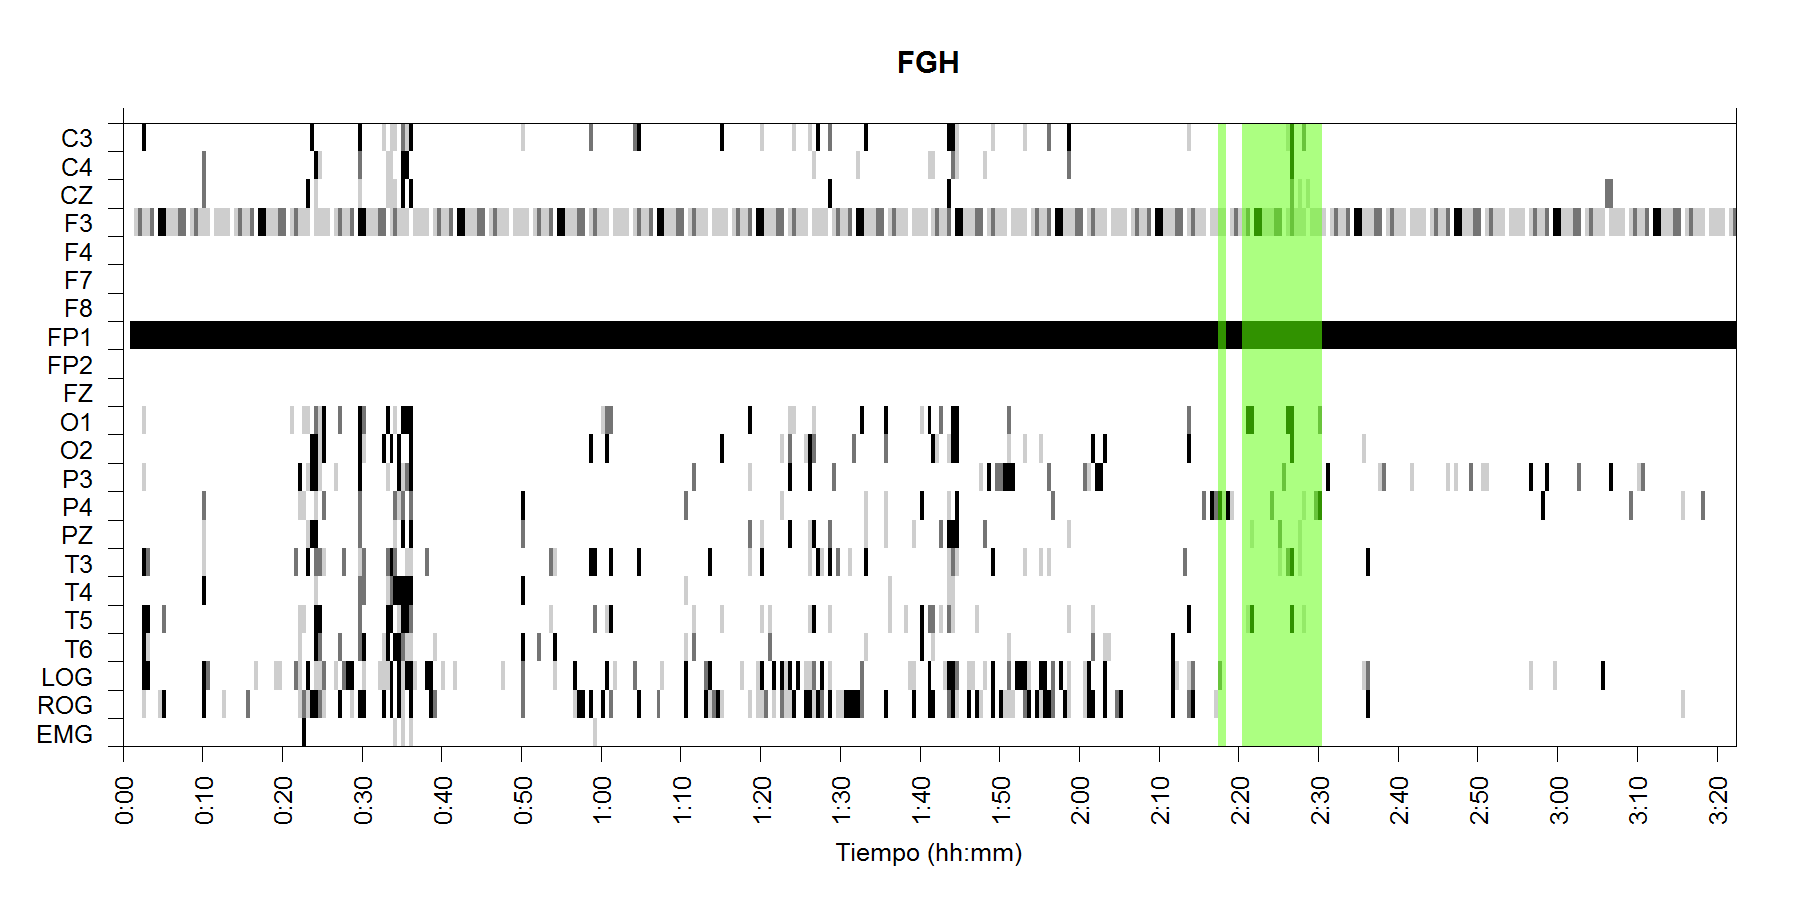
\includegraphics[width=0.95\linewidth]
{./img_ejemplos/FGHSUE_est.png} 
\caption{Compilado gr\'afico para el sujeto FGH; n\'otese el patr\'on inusual (completamente 
blanco o negro) en los canales correspondientes a la regi\'on frontal}
\label{FGH_especial}
\end{figure}

%%%%%%%%%%%%%%%%%%%%%%%%%%%%%%%%%%%%%%%%%%%%%%%%%%%%%%%%%%%%%%%%%%%%%%%%%%%%%%%%%%%%%%%%%%%%%%%%%%%
%%%%%%%%%%%%%%%%%%%%%%%%%%%%%%%%%%%%%%%%%%%%%%%%%%%%%%%%%%%%%%%%%%%%%%%%%%%%%%%%%%%%%%%%%%%%%%%%%%%

\subsection{Efecto del tama\~no de las \'epoca}

El uso de \'epocas de 30 segundos est\'a motivado por las recomendaciones de la AASM para 
clasificar, de manera estandarizada, las etapas de sue\~no a partir de registros de PSG 
\cite{AASM07}. 
No se discutir\'an en este trabajo motivaciones o evidencia para usar esta longitud de \'epoca en 
particular, ni para el caso contrario, sino que se acepta por fines de comparabilidad. 
Sin embargo, en alg\'un momento de este trabajo se usaron los registros de PSG organizados en 
\'epocas de 10 segundos de duraci\'on, como se muestra en la figura \ref{epocas_diferentes}. 
Se realizaron todos los an\'alisis descritos usando esta segmentaci\'on mixta (algunos sujetos con 
\'epocas de 10 s, otros con \'epocas de 30 s) y se obtuvieron resultados seg\'un los cuales no hay 
diferencias significativas en ninguno de los an\'alisis. 
Por otro lado, la representaci\'on gr\'afica construida a partir de los mismos datos, organizados
en \'epocas de 10 s, cambia sustancialmente (ver figura \ref{comp_VCR}).

\begin{figure}
\centering
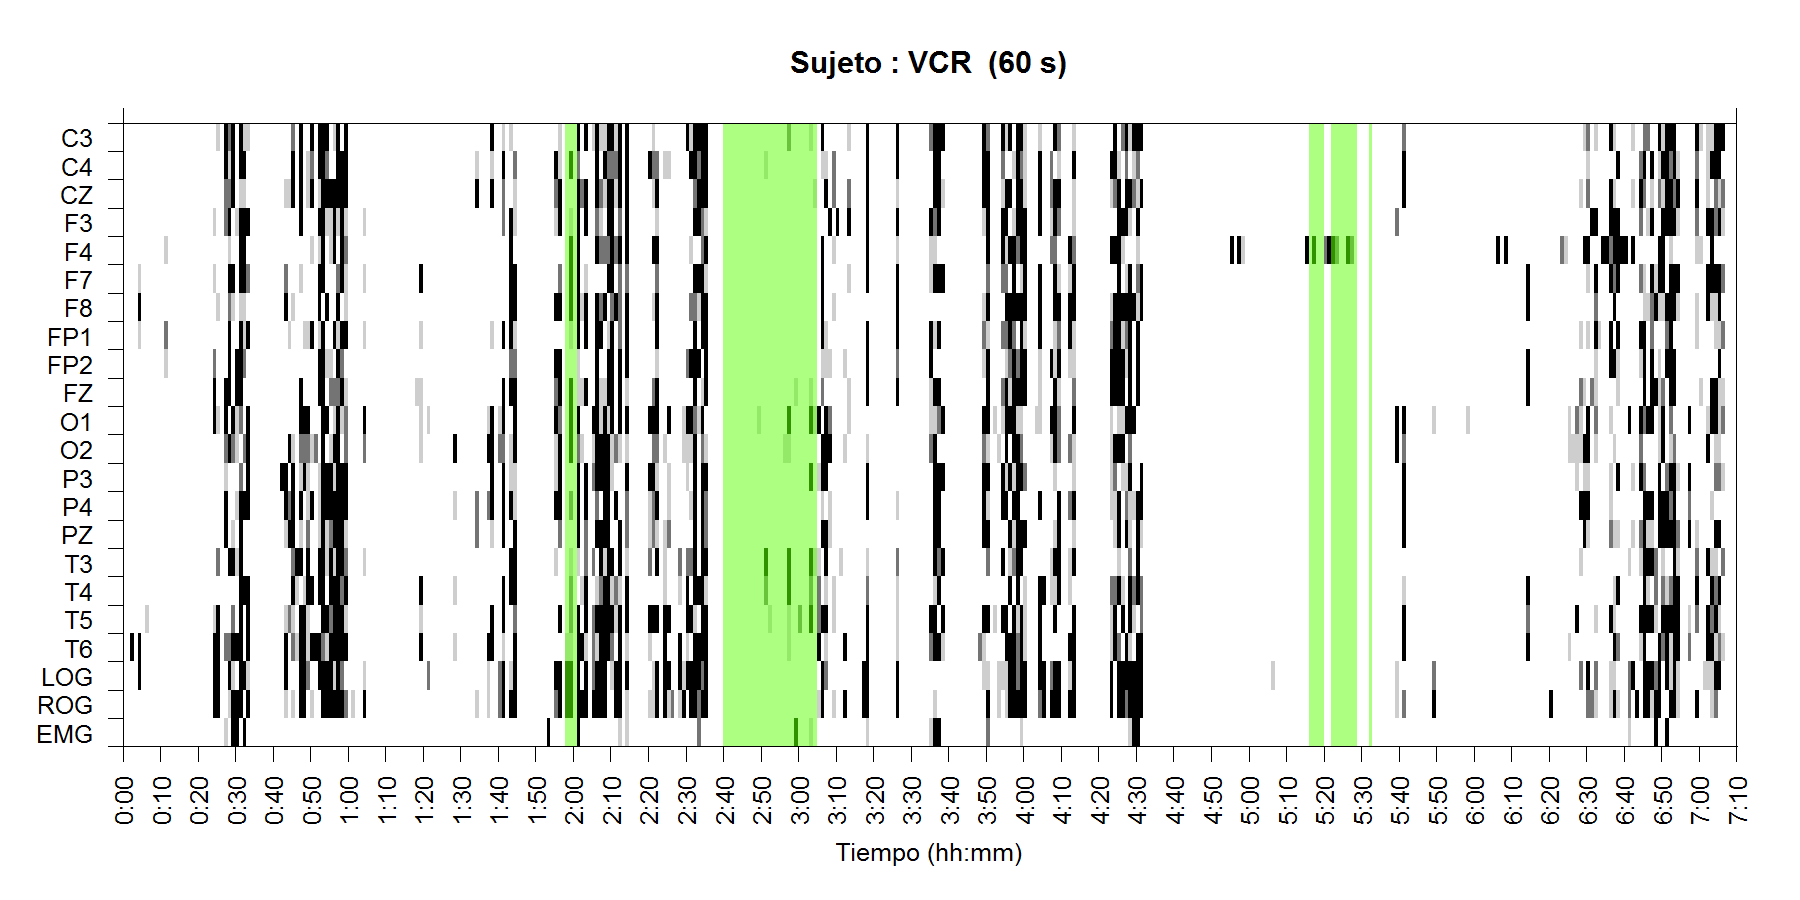
\includegraphics[width=0.9\linewidth] 
{./img_ejemplos/VCNNS1_est_60.png} 
\\
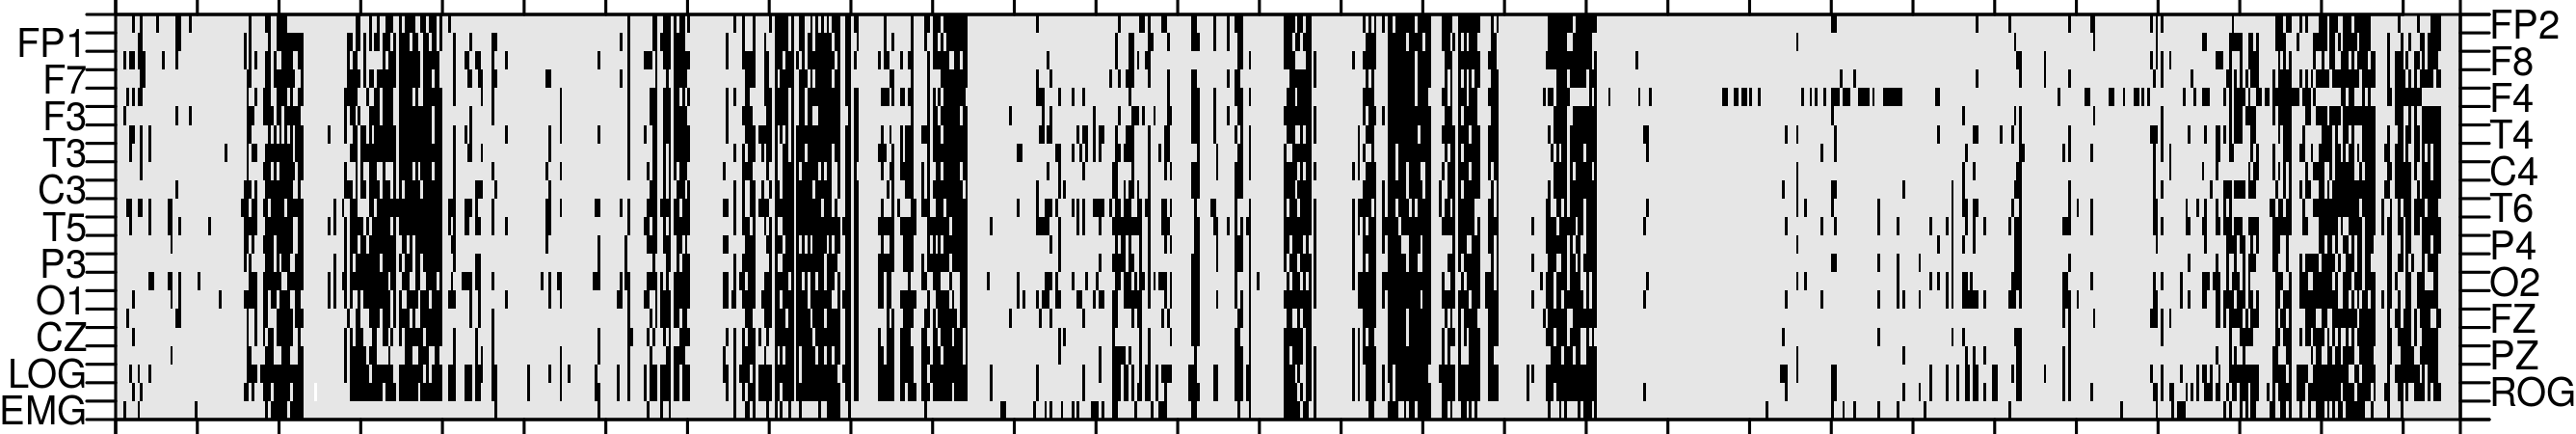
\includegraphics[width=0.9\linewidth]
{./img_ejemplos/VCNNS1_est_30.png} 
\\
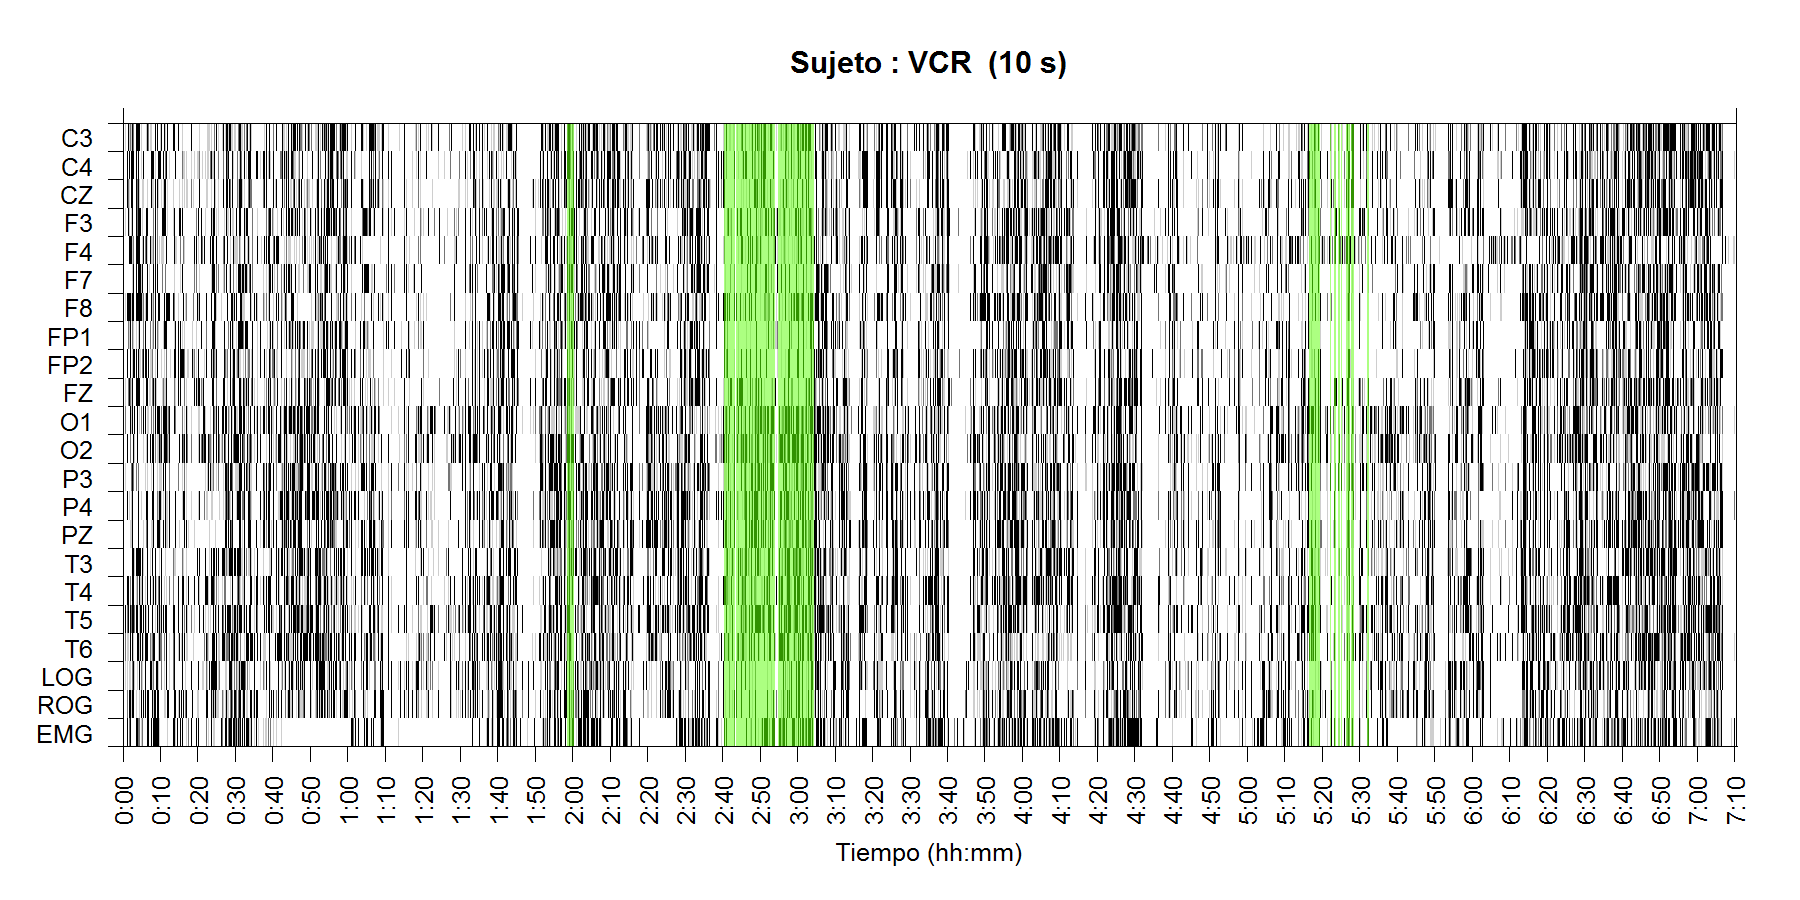
\includegraphics[width=0.9\linewidth]
{./img_ejemplos/VCNNS1_est_10.png} 
\caption{Compilaci\'on gr\'afica de las \'epocas clasificadas como PE, distribuidas en el tiempo
para cada uno de los canales. El registro corresponde al sujeto VCR, organizando el registro en
\'epocas de diferente duraci\'on}
\label{comp_VCR}
\end{figure}

El hecho de que los resultados fueran afectados de manera contundente por la forma en que se 
organizan los datos, sugiere que ser\'a provechoso prestar mayor atenci\'on a la naturaleza de las 
caracter\'isticas estudiadas y su posible interpretaci\'on en la fisiolog\'ia.
Se propone que los registros de PSG tienen una propiedad referida como 'estacionariedad local',
concepto introducido por Dahlhaus \cite{Dahlhaus97}.
A grosso modo, un proceso localmente estacionario es aqu\'el cuya FDE (que puede depender del 
tiempo) puede ser aproximada 'a trozos': usando FDE's correspondientes a procesos que poseen una 
representaci\'on espectral de Cram\'er y que est\'an 'correctamente ensamblados'.

%\begin{defn}[Estacionariedad local]
%Una secuencia de procesos estoc\'asticos de media cero, $\{ X_{t,N} \}$ con $t = 1, 2, \dots, N$, 
%se dicen localmente estacionarios en el tiempo $t_0 \in [0,1]$ si existe una representaci\'on del 
%tipo
%\begin{equation*}
%X_{t,N} = \intPI \widetilde{A_{t,N}}(\omega) e^{i \omega t} dZ(\omega)
%\end{equation*}
%donde se satisface que:
%\begin{itemize}
%\item $\{ Z(\omega) \}$ es un proceso de media cero con incrementos ortogonales, es decir
%\begin{equation*}
%\Cov{dZ(\omega_1),dZ(\omega_2)} =
%\begin{cases}
%d\omega &\text{, } \omega_1 = \omega_1 \\
%0 &\text{, otro caso}
%\end{cases}
%\end{equation*}
%\item Existe una constante $K$ y una funci\'on suave 
%$A: [0,1]\times [-\pi,\pi] \rightarrow \mathbb{C}$, 
%con $A(t_0,\omega) = \overline{A(t_0,-\omega)}$, tal que para toda $N$
%\begin{equation*}
%\sup_{\nicefrac{t}{N}\in \varepsilon_N(t_0)} 
%\sup_{\omega} \abso{ \widetilde{A_{t,N}}(\omega) - A(t_0,\omega) }
%\leq \frac{K}{N}
%\end{equation*}
%con $\varepsilon_N(t_0)$ es una vecindad de $t_0$ 
%tal que $\abso{\abso{\nicefrac{t}{N}-t_0}} = O(N^{-\alpha})$,
%%cuyo tama\~no es del orden $O(N^{-\alpha})$,
%con $0\leq \alpha < 1$
%\item $A(t_0,\omega)$ es continuo en $\{ t_0 \} \times [-\pi,\pi]$
%\end{itemize}
%\label{est_local}
%\end{defn}

Se propone que los registros de PSG se comportan como procesos localmente estacionarios; m\'as 
a\'un, esta caracter\'istica podr\'ia cambiar en adultos mayores con y sin PDC. 
Una motivaci\'on fisiol\'ogica para la hip\'otesis anterior es el contenido de los registros de
PSG: un conjunto descoordinado y homog\'eneo de ondas cerebrales, complejos K y husos de sue\~no.
Si bien esta composici\'on sugiere que la no-estacionariedad es la opci\'on m\'as obvia, el
an\'alisis llevado a cabo revela que el contenido de estos eventos no es homog\'eneo durante el
sue\~no; m\'as a\'un, mientras m\'as peque\~no sea el intervalo de tiempo observado, es m\'as
posible encontrar zonas de composici\'on m\'as o menos homog\'enea que puedan ser clasificadas
como PE.
Esta hip\'otesis explicar\'ia el cambio observado al cambiar el tama\~no de la \'epoca; de manera
arriesgada, se podr\'ia concluir que, entre los individuos con PDC, la homogeneidad del PSG es muy
similar durante MOR y NMOR.

%%%%%%%%%%%%%%%%%%%%%%%%%%%%%%%%%%%%%%%%%%%%%%%%%%%%%%%%%%%%%%%%%%%%%%%%%%%%%%%%%%%%%%%%%%%%%%%%%%%
%%%%%%%%%%%%%%%%%%%%%%%%%%%%%%%%%%%%%%%%%%%%%%%%%%%%%%%%%%%%%%%%%%%%%%%%%%%%%%%%%%%%%%%%%%%%%%%%%%%

\section{Conclusiones}

En registros de PSG para adultos mayores, segmentado en \'epocas de 30 segundos, la presencia 
proporcional de estacionariedad d\'ebil es significativamente diferente durante el sue\~no MOR y 
NMOR.
Estas diferencia se pudieron observar en el grupo Control para los canales C3, C4, F7, F8, FP1, 
FP2, O2, P4, LOG, ROG; en el grupo con PDC s\'olo se detectaron estas diferencias para los canales 
LOG y ROG.
Estos cambios entre MOR y NMOR pueden explicarse 
\begin{enumerate}
\item en LOG y ROG por las caracter\'isticas propias  del sue\~no MOR
\item en el resto de los canales (para el grupo Control), porque se tratan de la 
regi\'on frontal, asociada a la toma de decisiones, as\'i como la regi\'on posterior, 
asociada con la integraci\'on
de informaci\'on
\end{enumerate}

El an\'alisis de estacionariedad sobre registros de PSG para un adulto mayor con par\'alisis facial 
fue capaz de se\~nalar este padecimiento, visto como una ausencia total de \'epocas estacionarias
en una regi\'on concreta.

Los resultados encontrados sugieren que es posible interpretar los cambios neurofisiol\'ogicos 
durante el deterioro cognitivo como un cambio en la estructura funcional del cerebro al transitar 
entre sue\~no MOR y NMOR: el cambio es menos acentuado durante el PDC, pues tienen proporciones 
estad\'isticamente similares de \'epocas clasificadas como PE.
Esta interpretaci\'on propuesta es consistente con \cite{Valeria}.

En otro \'ambito, los patrones visuales descritos, visibles al mostrar gr\'aficamente la 
distribuci\'on de \'epocas PE, predicen parcialmente con las \'epocas de sue\~no MOR clasificadas 
por un experto (cuando menos en el grupo Control).
Se propone que la representaci\'on gr\'afica pudiera ser usado como auxiliar en la clasificaci\'on 
de segmentos de registro seg\'un la etapa de sue\~no.

Se presenta evidencia seg\'un la cual los registros de PSG, al menos para adultos mayores, no 
corresponden a series de tiempo no-estacionarias sino a series localmente estacionarias; esta 
distinci\'on cobra importancia al momento de elegir el tama\~no de ventana (en el tiempo) usada 
para organizar los registros.

%%%%%%%%%%%%%%%%%%%%%%%%%%%%%%%%%%%%%%%%%%%%%%%%%%%%%%%%%%%%%%%%%%%%%%%%%%%%%%%%%%%%%%%%%%%%%%%%%%%
%%%%%%%%%%%%%%%%%%%%%%%%%%%%%%%%%%%%%%%%%%%%%%%%%%%%%%%%%%%%%%%%%%%%%%%%%%%%%%%%%%%%%%%%%%%%%%%%%%%

\section{Trabajo a futuro}

Los resultados principales de este trabajo, con vista al trabajo futuro, consiste en las 
diferencias encontradas entre el sue\~no MOR y NMOR, as\'i como los patrones visuales asociados con 
la aparici\'on de sue\~no MOR; tales caracter\'isticas s\'olo fueron presentes para el grupo 
Control. Si bien no constituyen propiamente marcadores de deterioro cognitivo, esta metodolog\'ia
podr\'ia extenderse para identificar tales marcadores.
Por ejemplo, un marcador conocido \cite{Becerra12} del deterioro cognitivo es el 'enlentecimiento' 
de la actividad cerebral, entendido como un cambio en la concentraci\'on de energ\'ia desde ondas 
r\'apidas a ondas lentas.
Para detectar la estacionariedad d\'ebil se ha usado prueba de Priestley-Subba Rao, basada en 
estimadores locales para la funci\'on de densidad espectral (FDE); estos mismos estimadores 
podr\'ian ser usados para corroborar si efectivamente existen diferencias en la FDE para registros 
de adultos mayores con y sin deterioro cognitivo. 

Finalmente, y como se mencion\'o anteriormente, los patrones visuales en la representaci\'on 
gr\'afica pueden tener un uso como caracter\'isticas auxiliares para la detecci\'on 
semi-autom\'atica de \'epocas MOR en registros de PSG; en ese sentido, cabe mencionar el caso de 
los sujetos excluidos del estudio, para los cuales estos patrones parecen no cumplirse. 
Es en principio posible que la identificabilidad del sue\~no MOR, a trav\'es de estos patrones, 
pudiera fungir como marcador cl\'inico.

%%%%%%%%%%%%%%%%%%%%%%%%%%%%%%%%%%%%%%%%%%%%%%%%%%%%%%%%%%%%%%%%%%%%%%%%%%%%%%%%%%%%%%%%%%%%%%%%%%%
%%%%%%%%%%%%%%%%%%%%%%%%%%%%%%%%%%%%%%%%%%%%%%%%%%%%%%%%%%%%%%%%%%%%%%%%%%%%%%%%%%%%%%%%%%%%%%%%%%%
%%%%%%%%%%%%%%%%%%%%%%%%%%%%%%%%%%%%%%%%%%%%%%%%%%%%%%%%%%%%%%%%%%%%%%%%%%%%%%%%%%%%%%%%%%%%%%%%%%%
%%%%%%%%%%%%%%%%%%%%%%%%%%%%%%%%%%%%%%%%%%%%%%%%%%%%%%%%%%%%%%%%%%%%%%%%%%%%%%%%%%%%%%%%%%%%%%%%%%%
